\documentclass[a4j,12pt,twoside]{jreport}

%%%%%%%%%%%%%%%%%%%%%%%%%%%%%%%%%%%%%%%%%%%%%%%%%
% パッケージ宣言
%%%%%%%%%%%%%%%%%%%%%%%%%%%%%%%%%%%%%%%%%%%%%%%%%
\usepackage{graphicx}
\usepackage{times}
\usepackage{selectp}
\usepackage{epsf}
\usepackage{style/epsbox}
\usepackage{style/mediabb}
%\usepackage{style/boites_exemples}
\usepackage{style/verbatimfiles}
\usepackage{here}
\usepackage{url}
\usepackage{fancyhdr}
\usepackage{fancyvrb}
\usepackage{style/algorithm}
\usepackage{style/algorithmic}
\usepackage{cite}
\usepackage[dvipdfmx, usenames]{color}
\usepackage{colortbl}

\usepackage{ascmac}
\usepackage{amsmath}
\usepackage{amsthm}
\usepackage{amssymb}
\usepackage{latexsym}

\usepackage{style/thesis}

%%%%%%%%%%%%%%%%%%%%%%%%%%%%%%%%%%%%%%%%%%%%%%%%%
% マクロ定義
%%%%%%%%%%%%%%%%%%%%%%%%%%%%%%%%%%%%%%%%%%%%%%%%%
\newcommand{\argmax}{\mathop{\rm argmax}}
\newcommand{\argmin}{\mathop{\rm argmin}}
\renewcommand{\bibname}{参考文献}

%% myマクロ
%\input{mymacros}

%% マージン設定
%\oddsidemargin=17mm
%\evensidemargin=-4mm

%%%%%%%%%%%%%%%%%%%%%%%%%%%%%%%%%%%%%%%%%%%%%%%%%
% 本文開始
%%%%%%%%%%%%%%%%%%%%%%%%%%%%%%%%%%%%%%%%%%%%%%%%%
\begin{document}
\newtheorem{defi}{Definition}[section]
\newtheorem{thy}{Theorem}[section]

\pagestyle{fancyplain}

%\pagenumbering{roman}

% タイトルページ
\newlength{\oldtextwidth}
\setlength{\oldtextwidth}{\textwidth}
\setlength{\textwidth}{40zw}
%!TEX root = ../../main.tex
% タイトルページ
%\documentclass[a4j,12pt]{jreport}
%\usepackage{graphicx}
%\usepackage{times}
%\usepackage{selectp}
%\usepackage{epsf}
%\usepackage{epsbox}
%\usepackage{graphicx}
%\usepackage{verbatimfiles}
%\usepackage{here}
%%\usepackage{url}
%\usepackage{fancyhdr}
%\usepackage{algorithm}
%\usepackage{cite}
%\usepackage{ascmac}
%\usepackage{amsmath}
%\usepackage{amsthm}
%\usepackage{amssymb}
%\usepackage{latexsym}

%\usepackage{thesis}
%\input{mymacros}

%\oddsidemargin=17mm
%\evensidemargin=-4mm

%\setlength{\textwidth}{40zw}
%\begin{document}

\thispagestyle{empty}
\setcounter{page}{0}

%%%%%%%%%%%%%%%%%%%%%%%%%%%%%%%%%%%%%%%%%%%%%%%%%
% 定義
%%%%%%%%%%%%%%%%%%%%%%%%%%%%%%%%%%%%%%%%%%%%%%%%%

% タイトル
\def \title{MissionForest: 組織内外における\\協働支援のためのタスク構造化システムの試作}

% 著者
\def \author{後藤~誉昌}

% 提出日
\def \date{\today}

% 指導教官名
\def \teacher{白松~俊}

% 指導教官の肩書き
\def \teacherrank{准教授}

% 所属
\def \belong{名古屋工業大学\\工学部 情報工学科}

% 入学年度
\def \year{23}

% 学籍番号
\def \regnum{24115054}

%%%%%%%%%%%%%%%%%%%%%%%%%%%%%%%%%%%%%%%%%%%%%%%%%
% 本文
%%%%%%%%%%%%%%%%%%%%%%%%%%%%%%%%%%%%%%%%%%%%%%%%%

\def\sizeLL#1{\Huge #1}
\def\sizeL#1{\LARGE #1}
\def\sizeM#1{\Large #1}
\def\sizeS#1{\large #1}

\def\REYrule{\hbox to 5cm{\leaders\hrule height 1pt\hfill}}
\newbox\REYbox
\def\announce#1{
  \setbox\REYbox=\hbox{\REYrule\quad{\Large\bf #1}\quad\raise3pt\REYrule}%
  \gdef\REYbigrule{\hbox to \wd\REYbox{\leaders\hrule height 1pt \hfill}}%
  \centerline{\raise3pt\REYrule\vspace*{2mm}\quad{\LARGE #1}\quad\raise3pt\REYrule}}
\def\endannounce{\par\centerline{\REYbigrule}}

\begin{titlepage}
 \begin{center}
 %\renewcommand{\baselinestretch}{1.0}
  \vspace*{5mm}
  \sizeLL{卒業論文}\\
  \vspace*{10mm}
  \begin{announce}{(題~~目)}
   \sizeL{\title}\\
  \end{announce}
  \vspace*{20mm}
  \sizeM{指導教員~~~~~}\sizeL{\teacher}\sizeM{~~\teacherrank}\\
  %\vspace*{40mm} % 題目が2行の場合
 % \vspace*{30mm} % 題目が3行の場合
 \vspace{10mm}
  \sizeM{\belong}\\
  \vspace*{10mm}
  \sizeM{平成 \year 年 4 月 入学}\\
  \vspace*{3mm}
  \begin{table}[H]
    \begin{center}
     \begin{tabular}{cl}
      \sizeM{(学籍番号)} & \sizeL{{\underline{~~ \regnum ~~}}} \\
      \sizeM{(氏~名)} & \sizeL{\underline{~~ \author ~~}} \\
     \end{tabular}
    \end{center}
   \end{table}
  \vspace*{10mm}
  \sizeS{(提出日:~\today)}
  % \sizeS{(提出日:\ ~平成28年2月8日)}
 \end{center}
\end{titlepage}

%\end{document}

\cleardoublepage

% タイトル以降用パラメータ
\setlength{\oddsidemargin}{17mm}
\setlength{\evensidemargin}{-4mm}
\setlength{\textwidth}{\oldtextwidth}

\cleardoublepage

%ここからページ数開始
\pagenumbering{arabic}

\include{part/cover}

% アブストラクト
\cleardoublepage
%\pagenumbering{roman}
%!TEX root = ../../main.tex
\chapter*{論文要旨}
\label{chap0}
\addcontent{論文要旨}
旋律歌唱や旋律聴取における3つの処理側面として,リズム,旋律線,調性がある\cite{hatano2007}.旋律線 (pitch contour) は旋律概形とも呼ばれ,大まかな音高の上下動を指す.調性は,調やコード進行を指す.これら3要素のうち,音楽未経験者の即興合奏を難しくするのは調性判断である.調性判断とは調の種類を判定することを指す.調性以外の旋律線やリズムについては,初心者でも比較的容易に直感的動作として表出できる.そのため,音楽未経験者が即興合奏を行いたい場合,例えば地域振興のために幅広い層の自由な参加を志向した音楽イベントなどであっても,音楽未経験者は手拍子など自由度が低い手段での参加に限られる.
本研究では,ユーザの調性判断をシステムが補うことで,音楽経験に乏しい人でも調性感を損なわず自在に即興合奏に参加できるようなシステムの開発を目指す.具体的には,ユーザが旋律線とリズムを身体動作で入力すれば,システムが背景楽曲のコード進行に応じて音高補正を行い,調性の制約を満たし不協和にならない合奏ができる演奏インタフェースの実現を目指す. 
そのために,(1) 直感的な身体動作による旋律線やタイミング,音の種類などの入力手法,(2) 演奏音の出力範囲の指定手法,(3) 背景楽曲のコード進行に対する調性の制約の決定手法,の3つを課題として扱う.
(1)の直感的な入力手法としては,Intel RealSense 3D Camera (以下,RealSense) を用い,手の動きを認識して旋律線を入力する.RealSenseは手指のジェスチャー認識が容易であり,直感的な身体動作入力に適している.本研究では特に,認識誤りの多いtap動作の改善を試みた.
(2)の演奏音の出力範囲の指定手法は,手を伸ばし画面をスクロールさせるような操作モードを設け,手の深度によってこの操作モードを切り替える.
(3)の調性制約の決定手法は,能動的音楽鑑賞サービスSongle\cite{songle}のWeb APIからの解析情報を元に実現した.具体的にはSongleに公開されている100曲分について統計をとり,それをもとにコードに対する調性制約を決定した.
また,本研究で実装した改善版のtap認識,調性制約に対し,評価実験を行ったところ,tapの精度は実用的なものに向上,調性制約はコードの構成音のみと比べて意図通りの演奏がしやすく,不協和が少しあるという評価となった.
% \chapter*{Abstract}
\label{chap:Abstract-e}
\addcontent{Abstract}

Because of the spread of smartphones and the growth of the network technology, use of the social networking/micro-blogging service Twitter has spread widely. 
%スマートフォンの普及やネットワーク技術の発展により,Twitter などの SNS は 急速な成長を遂げた.
Social media such as tweets is attracting attention to its information value to know what they are doing and what they are thinking. 
%個人が用意に情報を発信できるため,一般の人々が何をして いるのか,何を思っているのかなど情報源としての価値も注目されつつあるそ
In recent years, a demand of society for analyzing topics in Twitter has been increasing.
 %そのような背景に伴い,近年,Twitter における話題分析のための技術に対する社会的要請は高まってきている.
However, so far, a usage scenario where users hark back to past event through browsing past timeline of Twitter has not been considered. 
%しかしながら,従来,過去のタイムラインをアーカ イブ化して振り返るような使い方は想定されていなかった
Therefore, we proposed a method of exploratory browsing for the past tweets set about a specific topic. 
%そこで,本研究では, ある話題に関する過去のツイート群における探索的閲覧手法を提案する

For a lot of tweets,  users cannot remember contents of the past tweets. It is difficult to determine an appropriate query for searching past tweets.
%大量に存在するツイート集合において,ユーザは過去にあった大量のツイートの内容を 知るはずもなく,何をクエリとして検索すればいいのか分からない.
In order to grasp the background of a specific topic, it is desirable to know time-series flows of features of tweets about the topic such as what events make trends of tweets changed.
%特定の話題 の背景を把握するためには,その話題に関するツイートの傾向がどのような流れ で移り変わっていったか,どのような出来事がツイートの傾向を変えたかという 時系列的な流れを知ることが望ましい.
Visualizing topics using a burst detection for Twitter is one of the researches about exploratory browsing for tweets.  
%ツイートに対する探索的閲覧の研究の中 でもバースト検出を利用したトピックの可視化などがあるが,
However, the method extracts only features from tweets in the burst period. In other words, it cannot extract features from tweets in all time.   
%従来の手法では盛り上がりのあった期間の特徴のみを抽出し,それ以外の期間の特徴が欠けてしまう
Presenting  features in only a particular time span, users cannot grasp detail information such as the changes of features in the time span.
%またある固定された区間の特徴のみをユーザに提示するだけでは,その区間 内の特徴の推移など,詳細な情報を把握することができない.
For users who lack knowledge about the retrieval object, these are not satisfied about the comprehensiveness of exploratory browsing. 
%検索対象に関する 知識の乏しいユーザにとって,これらは探索的閲覧における網羅性を満たしてい ない.

To solve these problems, we implemented an exploratory tweets browsing system which can extract feature terms from each time period, in a day or in a week or in a month,  using the statistical method combining Information Gain and Pointwise Mutual Information.
%そのために,本研究では,日,週,月の異なるタイムスケール毎にツイート を分割し,それぞれの期間内ツイート群から,統計的手法である情報利得と自己 相互情報量を用いた特徴語抽出を実現,
The system enables users to browse overview of tweets changing time scale and figure out the features of tweets along time-series.
%ユーザが動的にタイムスケールを調整 しながら閲覧することで,時系列に沿ったツイートの探索が可能な探索的閲覧支 援システムを開発した
We proposed Bias-Penalized Information Gain which can exclude inadequate terms that a specific user has frequently posted. We showed the effectiveness of the method by experimental results.
%また,期間の特徴語として不適切な語を除外するための バイアス罰則付き情報利得を提案し,実験からその有効性を示した.
Moreover, we confirmed that the exploratory browsing method we proposed is effective in recognizing a causal relationship between events and  opinions in a lot of past tweets by the experiment of tracking topics using the system.
%さらに,本 システムを利用した話題追跡の実験結果から,本研究での探索的閲覧手法が,過 去の大量のツイート群に対し出来事や意見などの時系列的な因果関係の把握に有 効であることを確認した.


\cleardoublepage

% 目次
% 目次
\markboth{目 次}{目 次}
\tableofcontents

% 図目次
\listoffigures
\markboth{図 目 次}{図 目 次}

% 表目次
\listoftables
\markboth{表 目 次}{表 目 次}
\cleardoublepage

% 序章
%!TEX root = ../../main.tex
\chapter{序論}
\label{chap:intro}

\section{本研究の背景}
音楽知識や音楽経験に乏しい人が音楽によるインタラクションを試みる際,調性感を損なわない音を発して参加することは非常に困難である.
実際に音楽未経験者が自由にかつ能動的に音楽インタラクションに参加する場合として,
地域社会振興のために開催される音楽イベント,アーティストのコンサート,などが考えられる.
従来,音楽経験の乏しい人がそのようなパフォーマンスに参加する手段は手拍子や掛け声,リズムに合わせて体を動かす程度のことに限られている,
波多野\cite{hatano2007}は旋律歌唱能力の発達過程や旋律聴取の認知的処理における3つの処理側面として,図\ref{img:hatano}に示すように,(1)リズム(rhythm),(2)旋律線(pitch contour),(3)調性(tonality)があるとしている.
(2)の旋律線とは音高の上がり下がりの運動パターンのことであり,初心者でもリズムやおおまかになら音が上がったか下がったかは比較的理解しやすい.(3)の調性とは文献\cite{ongakunotomo1979}によれば,広義には「支配的な中心音を有する音楽系」を指し,狭義には「長短調いずれかの主和音をもつ和声的な音楽系」を指す.調性は中心音,長調/短調,音階,和音などから説明され,音楽初心者が音楽について学ぼうとする場合,調性を理解することは最も大きな障害のひとつである.
よって調性は音楽未経験者が音楽活動を行おうとする際,苦手意識を持たれる原因となる.
この調性に関する知識の無さが引き起こす問題点を解決することで,誰でもより充実した音楽活動をすることが容易になると考えた.

\begin{figure}[t]
	\begin{center}
		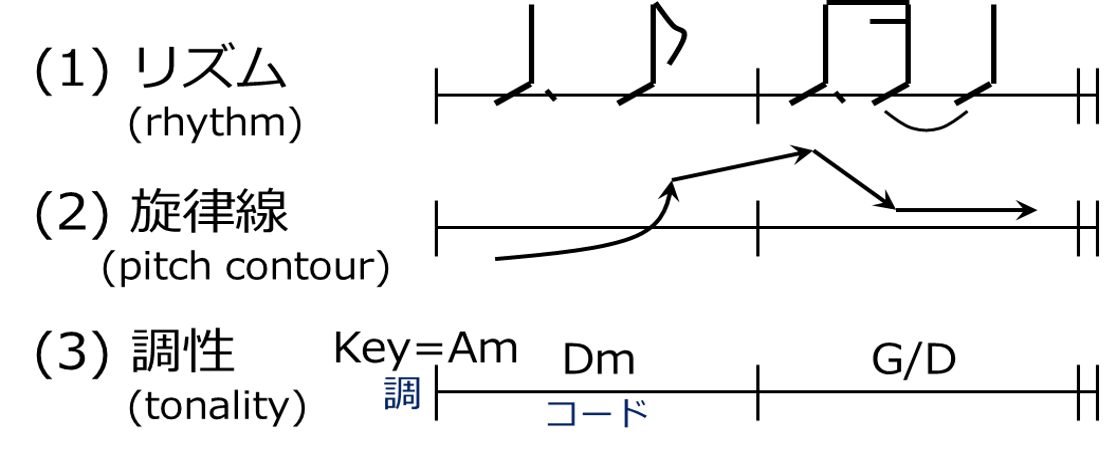
\includegraphics[width=0.9\linewidth]{./pics/01/hatano.png}
		 \caption{旋律歌唱や旋律聴取の認知的処理における3つの処理側面}
		\label{img:hatano} 
	\end{center}
\end{figure}
\section{本研究の目的}
本研究の目的は,ユーザーが直感的に操作できるように比較的知識を必要としないリズムと旋律線を身体動作で入力すれば,システムの音高補正により背景で流れている楽曲との調性の制約(以下,調性制約)に従って背景楽曲と協和を満たす演奏音を出力することで,音楽知識がなくても合奏ができる演奏インタフェースの実現である. 菅\cite{suga2008}は旋律線の手なぞりなどの身体動作が音楽理解を促進する方法として有効であるとしている.そのため旋律線の入力手段として身体動作を用いることは適切である.
本研究完成時には調性感を共有した演奏参加が可能になると期待される.コンサート会場で演奏される実楽曲の調や旋法と同期させた使い方を考えると,ステージ上のアーティストと聴衆のインタラクションのあり方を変える可能性があり,さらに,学校・保育施設での情操教育や福祉施設でのリハビリテーションにも活用できる可能性があり,幼児,児童,高齢者などのQOL向上に繋がると期待される.
また,旋律線とリズムを身体動作で入力することにより,ユーザーは演奏のための楽器を持ち運ぶ必要がなくなるため,演奏場所への移動距離や,スペースの制約に縛られることがない.
その操作性と音高の決定手法においていくつかの問題点ある.本研究ではそれらの問題を
(1)直感的な身体動作による旋律線やタイミング,音の種類などの入力手法.(2)演奏音の発音可能な音高範囲の指定.(3)調性制約の生成.の3つの課題として設定した.
\subsection{システム構成}
本システムのシステム構成を図\ref{img:sys_const}に示す.
まず,ユーザーはモーションセンサーの前でリズムと旋律線を身体動作で入力する.本研究ではモーションセンサーはIntel RealSense 3D Camera\footnote{http://www.intel.co.jp/content/www/jp/ja/architecture-and-technology/realsense-overview.html} (以下,RealSense)を使用した,RealSenseは手指の情報とジェスチャーを検出し,認識結果を本研究で実装する合奏支援システムに渡す.システム内部ではジェスチャーによるイベント切り替えや,手の座標とあらかじめ用意しておいた調性制約から背景楽曲と不協和音にならない演奏音を出力する.
\begin{figure}[t]
	\begin{center}
		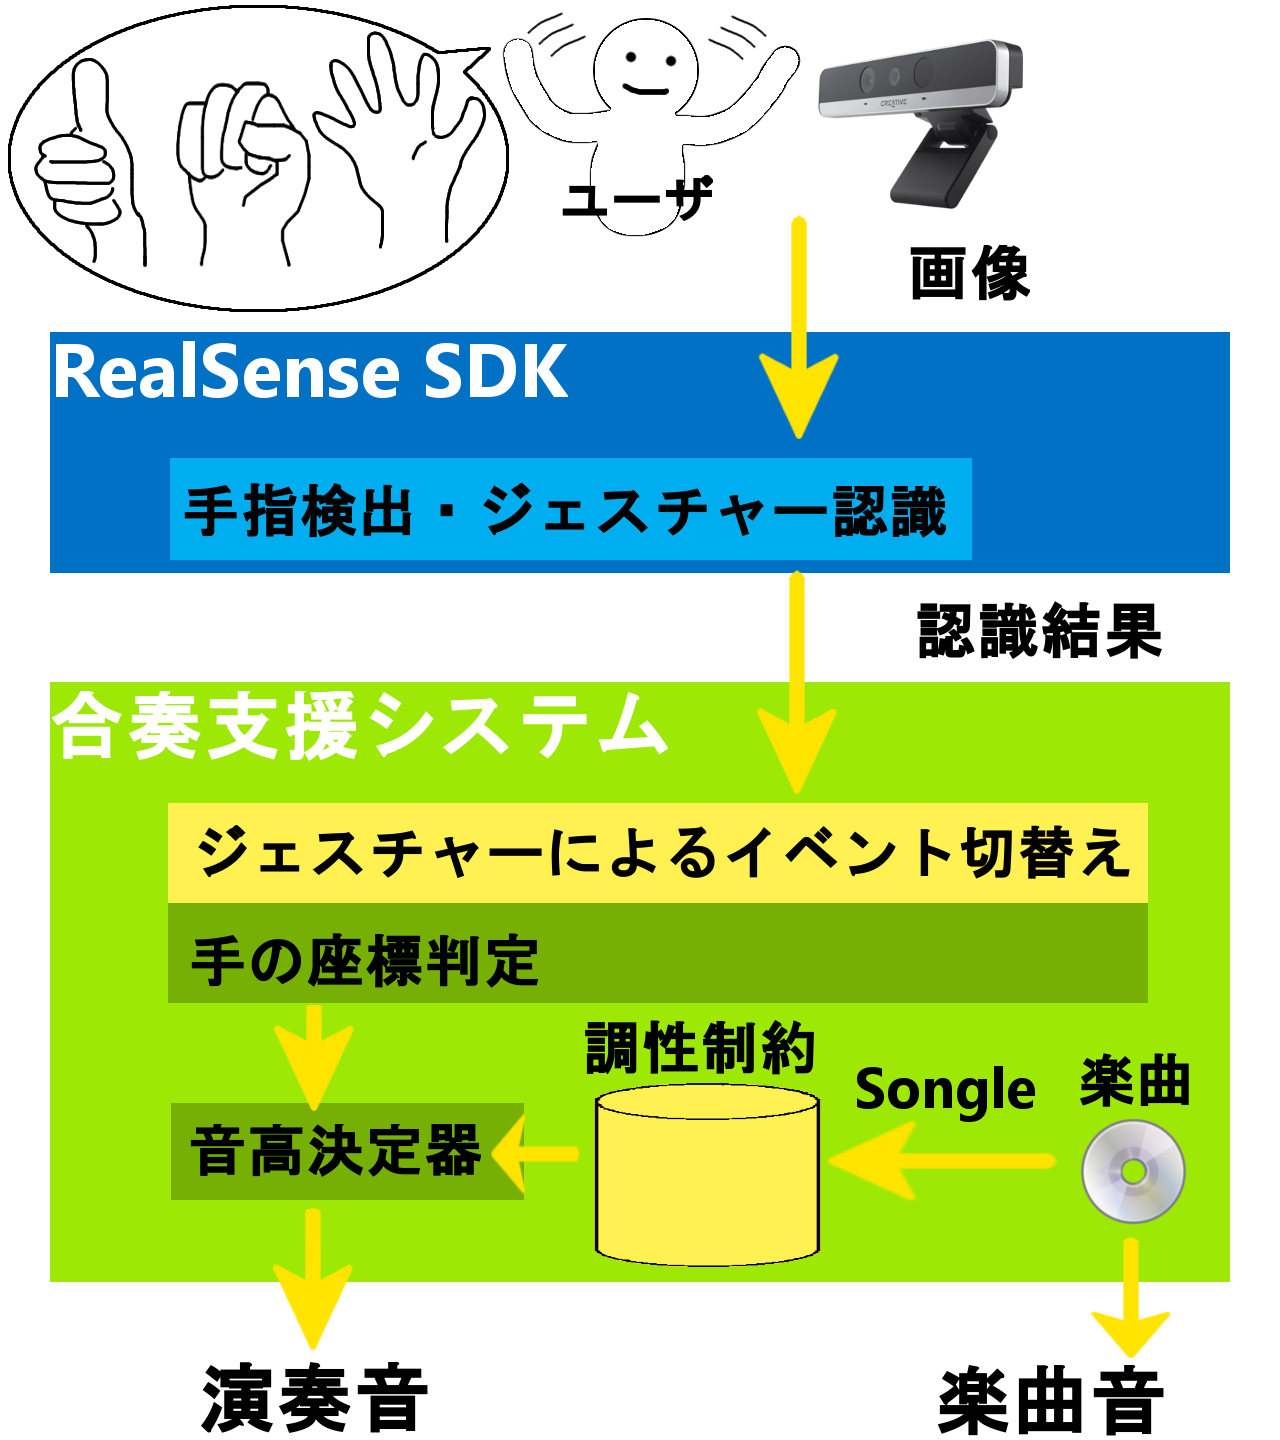
\includegraphics[width=0.9\linewidth]{./pics/01/system_configuration_diagram.png}
		\caption{システム構成図}
		\label{img:sys_const} 
	\end{center}
\end{figure}
\section{本論文の構成}
本論文の構成を以下に示す.第2章では関連研究や関連システムと本研究の動作・開発環境について述べる.第3章では直感的な身体動作とリズムの入力手法について述べる.第4章では演奏音の発音可能な音高範囲の指定について述べる.第5章では調性制約の生成について述べる,第6章では前章までで述べたシステムの評価実験の結果をまとめ,第7章で本研究をまとめる.

\cleardoublepage

% 関連研究
%!TEX root = ../../main.tex
\chapter{動作・開発環境と関連研究}
\section{動作・開発環境}
本研究の動作・開発環境について述べる.

\subsection{Intel RealSense 3D Camera}
旋律線とリズムの直感的な入力手段として使用した.RealSenseは手指やジェスチャー,顔の部位や表情,心拍や音声,対象物の奥行きなどを認識することができる.さらに,今後各国の主要PCメーカーがRealSenseを内蔵したPCを発売することに賛同している.従来,Kinect\footnote{http://www.xbox.com/ja-JP/kinect}をはじめとするモーションセンサ類を使用するにはわざわざデバイスを購入しなければならず,モーションセンサ類の存在を知らなかったり,存在を知っていても新たにデバイスを用意する手間や安価であっても購入の費用を嫌う人は一部のユーザーが使うものという認識であった.RealSense搭載PCの増加やWindows Helloなどモーションセンサでの開発経験のない一般ユーザーでも,容易に手に入ったり認知することができるRealSenseはその普及度においても期待されているデバイスである.

\subsection{Processing}
本システムの実装には,RealSense SDKを扱うことができ,画像や音声を比較的容易に行うことができるプログラミング言語Processingを用いる.Processing\footnote{https://www.processing.org/}は,MIT(Massachusetts Institute of Technology)メディアラボに所属していたCasey ReasとBen Fryによって開発された,視覚芸術のためのプログラミング教育ように作られたJavaをベースにした開発環境である.\cite{takahasi2010}
\section{関連研究}
本研究と関連のある研究やシステムを紹介する.

\subsection{Songle}
Songle\cite{songle}とは,音楽をサビ,メロディ,コード,ビートなどの構造を表示しながら鑑賞できるサービスで,ピアプロ\footnote{http://piapro.jp/}やSoundCloud\footnote{https://soundcloud.com/}の楽曲ページ,ニコニコ動画\footnote{http://www.nicovideo.jp/}やYouTube\footnote{https://www.youtube.com/}などにアップロードされている合法的に視聴可能な楽曲を音楽理解技術により自動解析しAメロ・Bメロ・サビといった繰り返し構造や、ビートの位置・コード進行・ボーカルの音高などを自動的に解析して見ることができる.さらにSongle上では複数のユーザでコンピュータの自動解析による誤差を訂正することで,解析結果の精度を高めている.また,Songle解析結果をJavaScriptから操作し,WEB上で利用するためのSongle Widget API\footnote{https://widget.songle.jp/}を用いることによって解析結果をJSONファイルとして参照することができる.

\subsection{KAGURA}
中村ら\cite{nakamura2010}はRealSenseを利用した音楽演奏アプリKAGURA\cite{kagura}を開発した.KAGURAはRealSenseを使用することによりRealSenseの特徴であるジェスチャー認識機能を利用し,身体動作で音の高さを,ジェスチャーで細かい設定や操作を指定することができる.出力される音は不協和音にならないようになっているため,適当に体を動かしたり,音楽演奏経験のない人でも音楽を演奏することができる.
また,KAGURAには録画機能とYouTubeへのアップロード機能が付いているため,気に入った演奏をすぐにインターネット上に公開することも容易に行えるようになっている.
\subsection{Airstic Drum}
菅家ら\cite{kanke2013}は,物理的に打面のあるドラム楽器(以下,実ドラム)の問題点を解決するために,実ドラムの補助として使用頻度の少ない打楽器に対して仮想ドラムを適用することで実ドラムと仮想ドラムの両方の利点を持ったAirstic Drumを設計した.この仮想ドラムの実装は無線通信機能を持つ加速度センサを搭載したドラムスティックから得られる加速度,角速度に閾値を設定し音の出力タイミングとしている.具体的には,加速度が設定された閾値(以下,基準強度)を超え,再び基準強度を下回るまでの経過時間の実ドラムと仮想ドラムの違いを識別して仮想ドラムの叩打タイミングとしている.また,仮想ドラムの叩打と演奏音の出力タイミングの時間差を測定するため,60bpm,90bpm,120bpmのテンポでメトロノームに合わせて仮想ドラムの叩打を繰り返し,メトロノームのクリック音とMIDI音源にメッセージが送信されるタイミングの時間差を計測した.

\subsection{調性理解モデルPFG Tonnetz}
白松ら\cite{shiramatsu2015}は調性理解モデルPFG Tonnetz (Prime Factor-based Generalized Tonnetz)を考案した.ある調の主音の周波数と協和音程の周波数比は,

\begin{align}
f=\Bigl(\prod_{pはn以下の素数} p^{(z_p)}\Bigr)\cdot f_{\rm tonic} ~~(z_pは整数)
\end{align}

のような素数の積で表すことができる.白松らは$n=5$と置いた上で,オクターブ隔たった音は音楽的に等価であることを考慮し,2の指数$z_2$軸をなくして$z_{3}z_{5}$平面へ投影すると,

\begin{figure}[t]
\begin{center}
	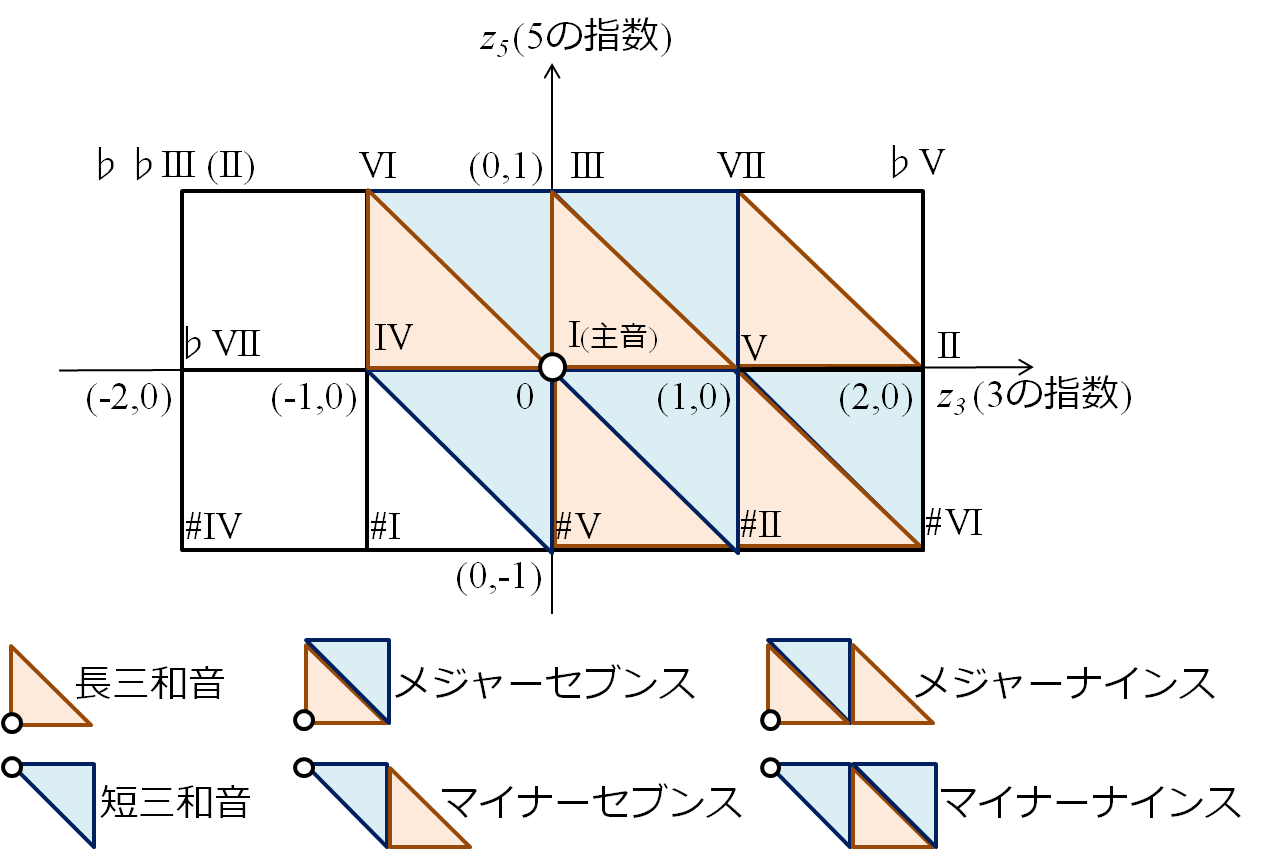
\includegraphics[width=0.9\linewidth]{./pics/02/pfg-tonnetz.png}
	\caption{調性理解モデル PFG Tonnetz (5-limit)\cite{shiramatsu2015}}
	\label{img:pfg-tonnetz} 
\end{center}
\end{figure}
図\ref{img:pfg-tonnetz}のように$z_3z_5$平面に配置される.この平面上の根音$(a,b)$に対して以下のような整数格子点列$\mathrm{chord}(a,b,\delta,m)$を考える.

\begin{align}
\mathrm{chord}(a,b,\delta,m)=\bigl[(a,b)+\sum_{i=0}^k \delta(i)\bigr]_{k=0,1,\cdots,m} \label{eq:code}\\
\delta_{\rm maj}(i)=\begin{cases}(0,1)&(iが奇数のとき)\\(1,-1)&(iが偶数のとき)\end{cases} \label{eq:maj}\\
\delta_{\rm min}(i)=\begin{cases}(1,-1)&(iが奇数のとき)\\(0,1)&(iが偶数のとき) \label{eq:min}\end{cases}
\end{align}

根音$(a,b)$を調の主音$(0,0)$で置き換えて考えると,明るい長音階の構成音(I, II, III, IV, V, VI, VII)が原点の上側$0 \leq z_5 \leq 1$に分布し,暗い短音階の構成音(I, II, \#II, IV, V, \#V, \#VI)が原点の下側$-1 \leq z_5 \leq 0$に分布するのが見て取れる.

このモデルは,音名,階名,コード名のようなシンボルを前提としては用いておらず,周波数比に基づく認知的原理のみから導かれる.まとめると,導出の過程で現れた以下の表現形式は,上記の認知的原理および導出されたモデルの観察から自然に導かれたものである.

\begin{itemize}
\item 整数格子点$(z_3, z_5)$: 音階の構成音,階名
\item 三角形$\bigl[(a,b)$, $(a,b+1)$, $(a+1,b)\bigr]$:\\
~~~ 整数格子点$(a,b)$を根音とする長三和音
\item 三角形$\bigl[(a,b)$, $(a+1,b-1)$, $(a+1,b)\bigr]$:\\
~~~ $(a,b)$を根音とする短三和音
\item 整数格子点列$\mathrm{chord}(a,b,\delta_{\rm maj},m)$:\\
~~~ $(a,b)$を根音とする長和音
\item 整数格子点列$\mathrm{chord}(a,b,\delta_{\rm min},m)$:\\
~~~ $(a,b)$を根音とする短和音
\end{itemize}

このPFG Tonnetzは数学者Leonhard Eulerが1739年に考案した調性理解モデルをもとに.
音楽学者Hugo Riemannが1880年に発展させたTonnetzというモデルに似ている
Tonnetzは1980年代以降,数学的に定式化された新リーマン理論(NeoRiemannian theory)へと発展し,様々な拡張が行われた\cite{behringer10}%\cite{tymoczko12}
が基本的には図\ref{img:euler},図\ref{img:riemann}のように音名同士を繋いだモデルであり,調の主音は表現できていない.
\begin{figure}[t]
	\begin{center}
		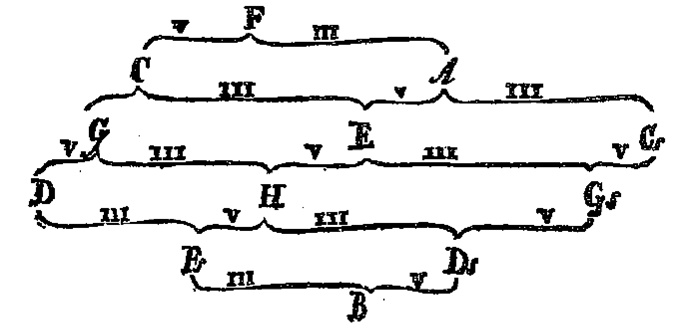
\includegraphics[width=0.9\linewidth]{./pics/02/Eulers_tonnetz.png}
		\caption{Eulerの調性理解モデル\cite{shiramatsu2015}}
		\label{img:euler} 
	\end{center}
\end{figure}
\begin{figure}[t]
	\begin{center}
		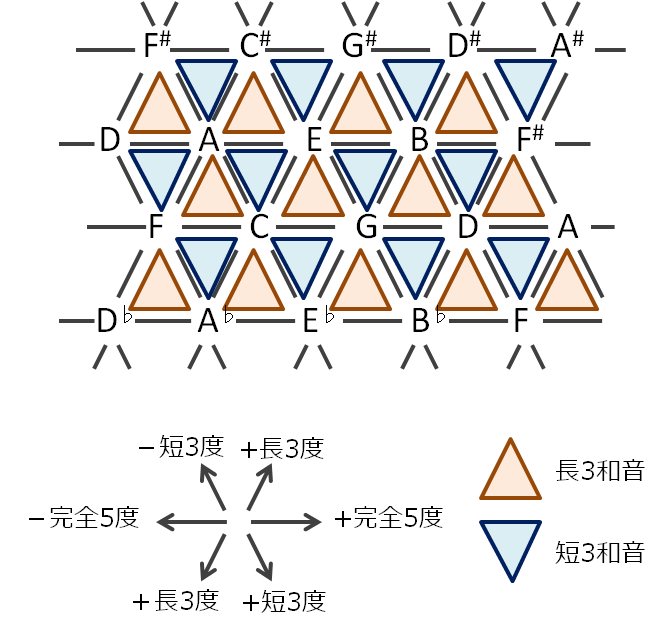
\includegraphics[width=0.9\linewidth]{./pics/02/tonnetz_vertical.png}
		\caption{Riemannの調性理解モデル\cite{shiramatsu2015}}
		\label{img:riemann} 
	\end{center}
\end{figure}


\cleardoublepage

% 期間毎の特徴語抽出手法
\chapter{直感的なリズムと旋律線の入力手法}
本章では身体動作で直感的にリズムと旋律線を入力する手法について述べる.

\section{RealSense SDK}
RealSenseを扱うためのRealSense SDKが提供する機能のうち,本研究で使用したものを述べる.
\subsection{RealSenseのジェスチャー認識}
RealSense SDKでは,図\ref{img:jesture}に示す11種類のジェスチャーが定義されている.しかし,あらかじめ定義されているジェスチャーの多くは,認識精度に問題があり,認識漏れや遅延が発生する.音楽を演奏するインタフェースの操作手段としてジェスチャーを使用するにはこの遅延が大きな障害となる.本研究ではジェスチャー認識に加えて,手指や手のひらの座標,開閉度などのパラメータを利用して認識精度を向上させた.
\begin{figure}[t]
	\begin{center}
		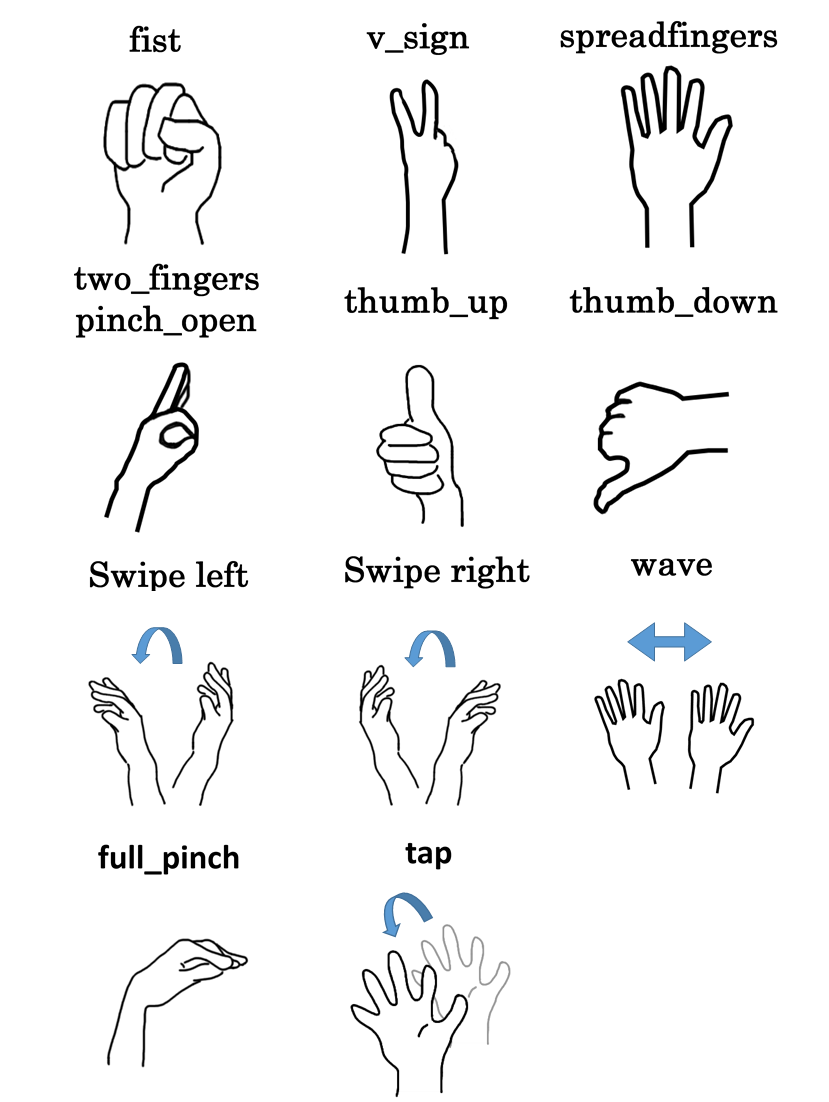
\includegraphics[width=0.9\linewidth]{./pics/03/jesture.png}
		\caption{11種類のジェスチャー}
		\label{img:jesture} 
	\end{center}
\end{figure}

\subsection{関節の認識}
RealSenseカメラでは図\ref{img:handlabels}に示す22種類の手のひらの関節を認識することができる.本研究では図\ref{img:handlabels}のMiddle Fingertipの座標を指先の座標,Palmの座標を手のひらの座標として扱った.
\begin{figure}[t]
	\begin{center}
		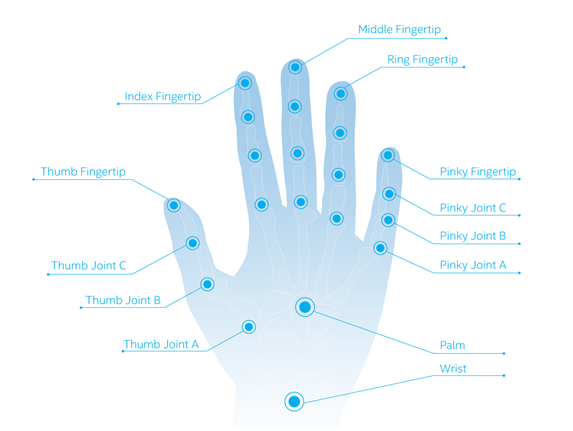
\includegraphics[width=1\linewidth]{./pics/03/hand_labels.png}
		\caption{22種類の関節\cite{hand_labels}}
		\label{img:handlabels} 
	\end{center}
\end{figure}

\section{持続音と減衰音}
持続音とはバイオリン,笛などのような音量が一定のまま鳴り続ける音で,減衰音とはピアノ,鉄琴,木琴などのような音量が減衰していく音である.
本研究ではユーザの演奏表現にバリエーションを提供するために持続音と減衰音の両方を扱う.よってユーザーが好きな時に持続音と減衰音を切り替えられるように,図\ref{img:jesture}のうちthumb\_up動作をすると演奏音が持続音か減衰音に切り替わるように割り当てた.
本研究では左右の手で出力される演奏音は独立しており,2和音まで出力可能である.

\subsection{旋律線の入力}
図\ref{img:note1}に身体動作による旋律線の入力の概要を示す.ジェスチャーで音の種類を持続音に指定しユーザーはRealSenseの前で動くと指先の座標の時間的変化がそのまま旋律線として入力される.Processing側では画面を現在発音可能な演奏音の数で等分割した領域を用意して,インタフェースの画面に色分けして表示する.手指の座標がどの領域に存在するかにより,その領域とひも付けられた背景楽曲の調性制約を満たす周波数の音が演奏音として出力される.
\begin{figure}[t]
	\begin{center}
		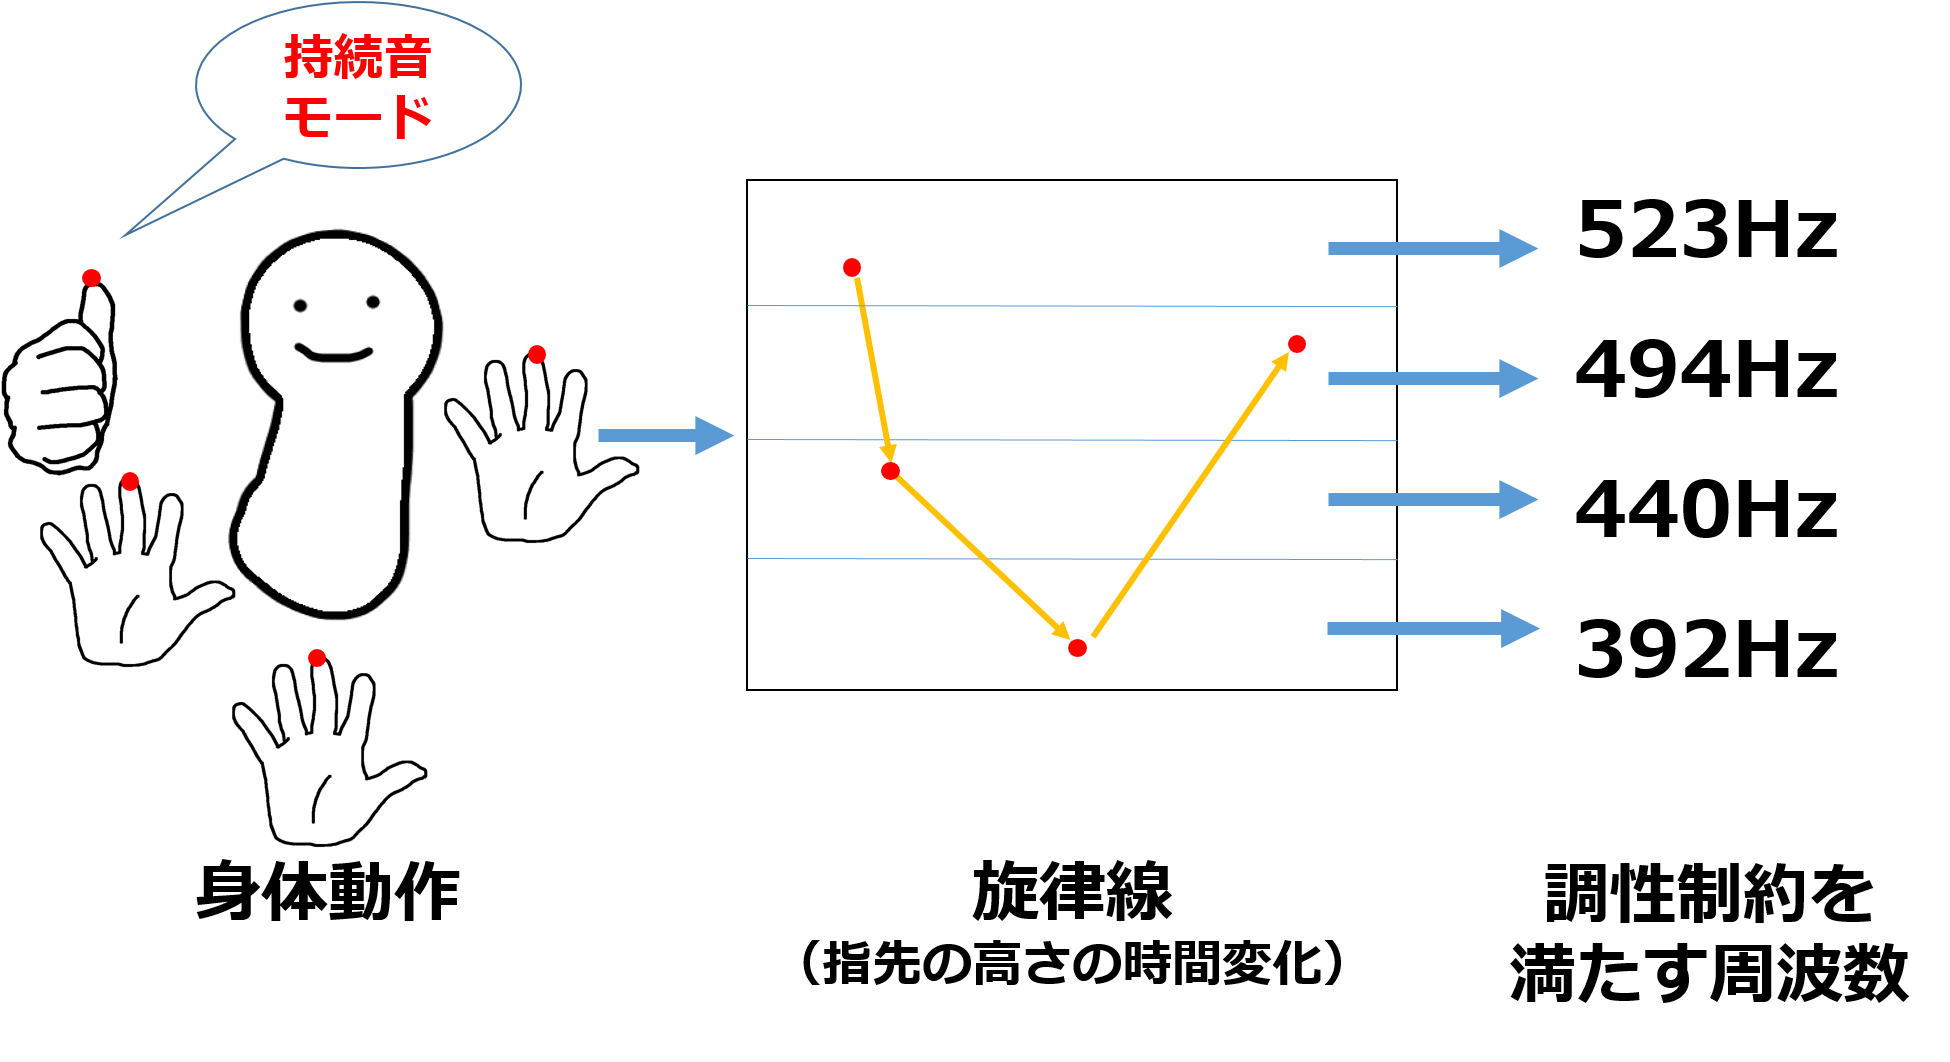
\includegraphics[width=0.9\linewidth]{./pics/03/in_note.png}
		\caption{直感的な旋律線の入力方法}
		\label{img:note1} 
	\end{center}
\end{figure}
\subsection{リズムの入力}
持続音を出力する際に現在演奏している音の領域と離れた領域の音を出力する場合,手を移動させた時に通った領域の音まで出力してしまう.そこでSongle Web APIから取得した背景楽曲の拍に合わせて点滅する円を画面に表示させ,リズムを取りやすくするとともに,円が表示されてないタイミングのとき演奏音をportamentoを設定することで,離れた領域の音を出力するときに間の領域の音を出力するのを防ぐ.本研究では点滅する円に合わせるようにして手を動かすことをリズムの入力とした.図\ref{img:portamento}に拍とportamentoのタイミングを示す.曲のビート一拍分を半分に分けた時の前半部分の間に円を表示させ,後半部分の間に円を非表示にしてportamentoを設定する.後半部分の間指先を動かして領域を移動すると,出力音は滑らかに変化する.
\begin{figure}[t]
	\begin{center}
		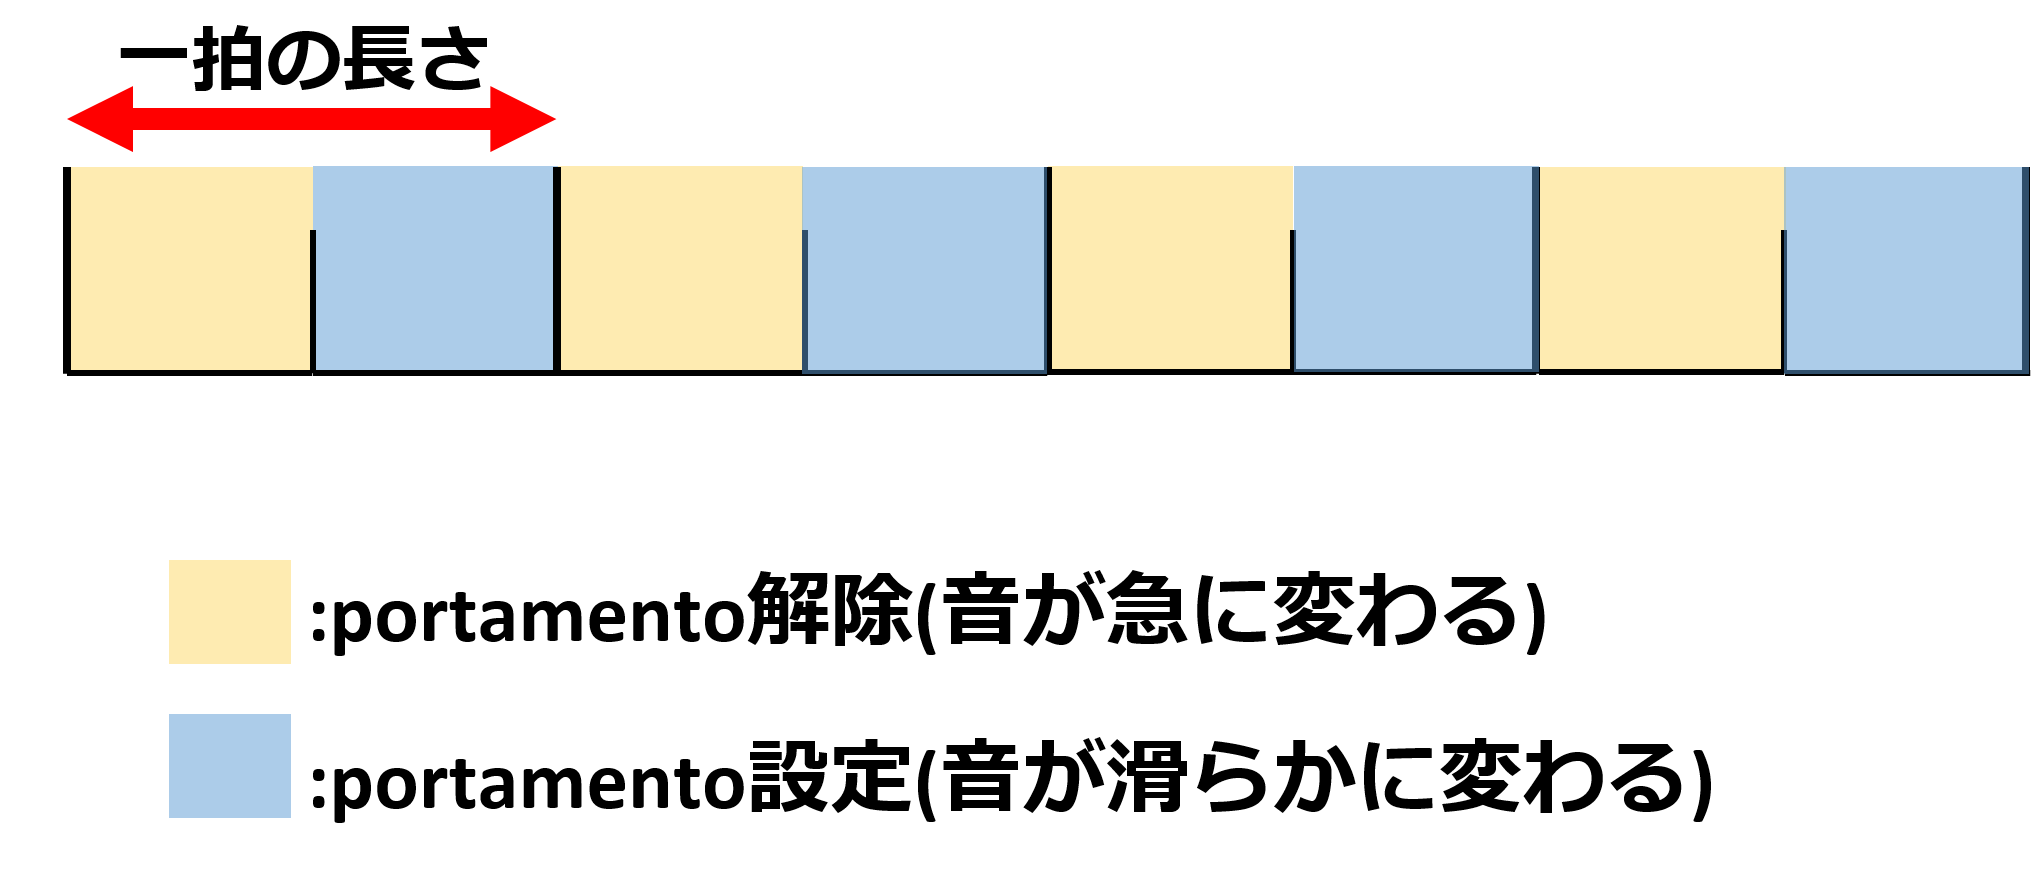
\includegraphics[width=1\linewidth]{./pics/03/portamento.png}
		\caption{拍とportamentoのタイミング}
		\label{img:portamento} 
	\end{center}
\end{figure}
\subsection{持続音のジェスチャー}
持続音のオンセットとオフセットには,それぞれ図\ref{img:jesture}のspreadfingersとfistを割り当てた.これらのジェスチャーの精度を向上させるため,指の開閉度というパラメータ(0〜100)を利用した.ジェスチャー認識の条件に開閉度が90以上の時,spreadfingers動作を,1fあたりの変化量が-10を下回った時,fist動作をするように設定させた.
\subsection{減衰音のジェスチャー}
減衰音のオンセットには図\ref{img:jesture}のtap動作を割り当てた.本研究の持続音は1秒間だけ出力されるので減衰音のオフセットにジェスチャーは割り当ててない.tap動作をしたとき指先の座標が存在する領域に対応した周波数の音が出力される.tap認識の精度を向上させるため,指先と手のひらの速さと移動距離に閾値を設定したときtap動作をしたと認識させた.図\ref{img:tap}に閾値を設定した場所を示す.閾値は経験的に指先のz座標のカメラ方向への移動距離が20mm以上移動した時,指先の3次元移動速度が1.8m/s以上,手のひらの移動速度が0.6m/s以上1.5m/s以下の時tap動作とした.本研究のtap動作はRealSense SDKのtap認識の代わりに使用しているため,どちらが優れているかの評価実験を行い,第6章でまとめた.
\begin{figure}[t]
	\begin{center}
		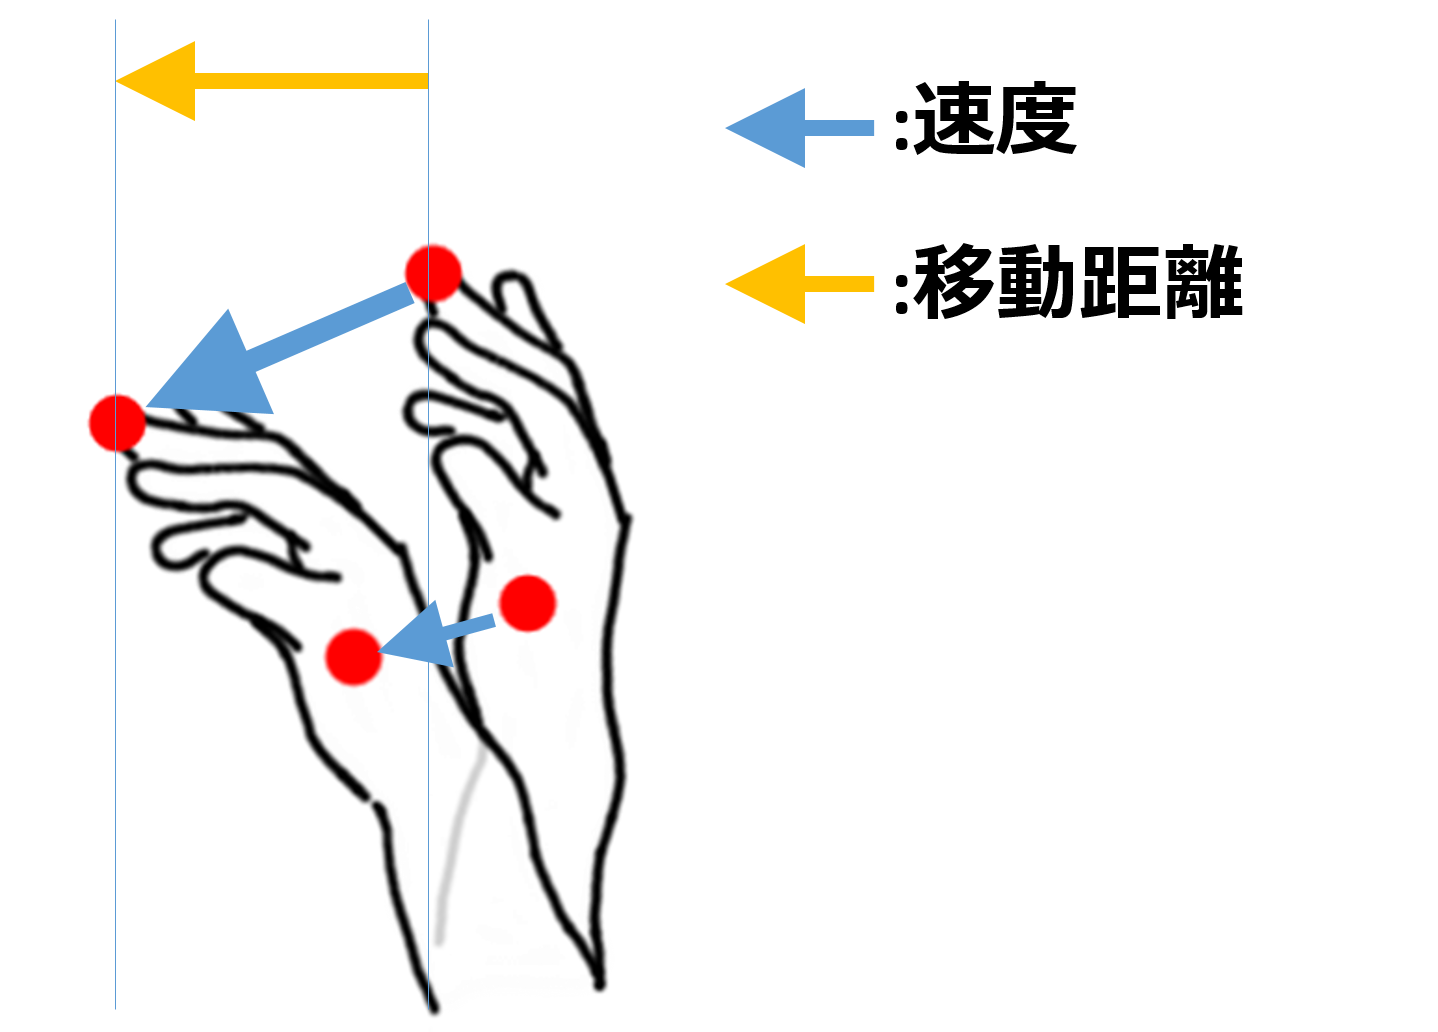
\includegraphics[width=1\linewidth]{./pics/03/tap.png}
		\caption{tap動作の閾値}
		\label{img:tap} 
	\end{center}
\end{figure}
\subsection{実行結果}
図\ref{img:interface_result1},図\ref{img:interface_result3}に実行結果を示す.画面下の拍によって点滅する円である.指先の小さい円が指先の座標を表し,領域の色が濃くなっているところが現在指定している高さの領域である.赤になるほど音が高く,緑になるほど音が低くなる.
\begin{figure}[t]
	\begin{center}
		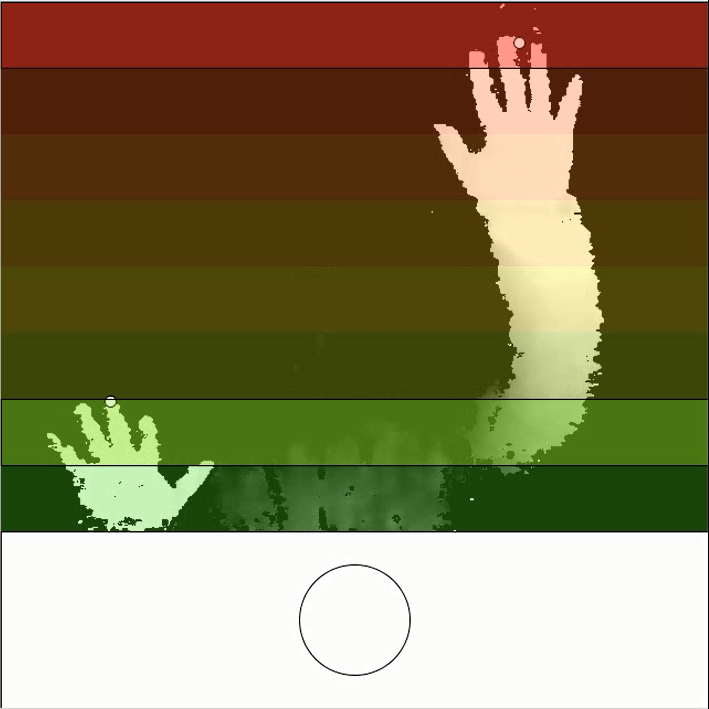
\includegraphics[width=0.5\linewidth]{./pics/03/result1.png}
		\caption{実行結果1}
		\label{img:interface_result1} 
	\end{center}
\end{figure}
\begin{figure}[t]
	\begin{center}
		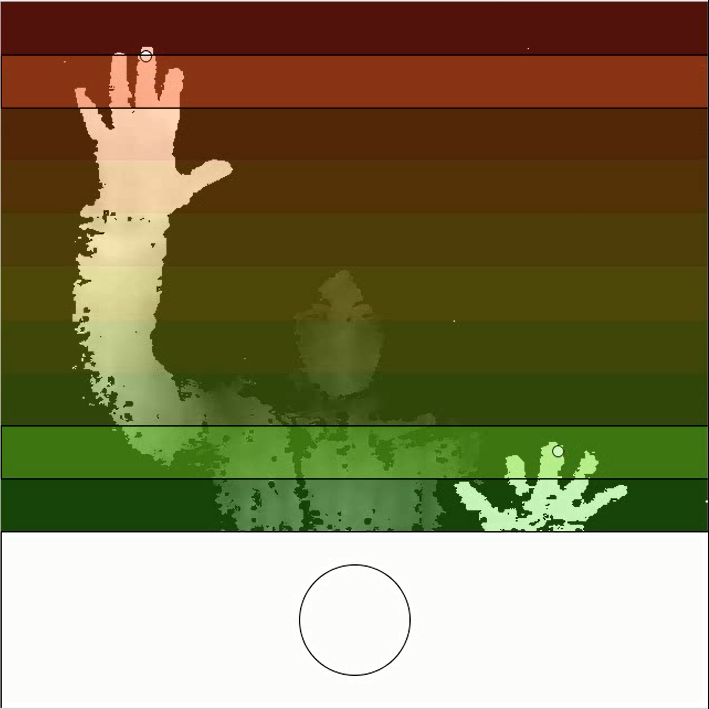
\includegraphics[width=0.5\linewidth]{./pics/03/result3.png}
		\caption{実行結果2}
		\label{img:interface_result3} 
	\end{center}
\end{figure}

\cleardoublepage

% タイムスケールを考慮した時系列的話題追跡
\chapter{演奏音の発音可能な音高範囲の指定}
演奏音の発音可能な音高範囲(以下,音高範囲)を指定する手法について述べる.

\section{実装手法}
RealSenseで扱えるカラー画像の最大サイズは1920$\times$1080である.しかし本研究では主に深度画像を扱うため深度画像の最大サイズ640$\times$480がインタフェースの画面サイズとなる.
本研究のインタフェースは現在発音可能な音を,画面のサイズを音の数で均等に分けて色分けされた領域で表示している.
出力する音の数が多くなるほど一つの音の領域が狭くなり,望む領域に指先を合わせづらくなるため出力できる音高範囲を2オクターブまでとしている.
これによって演奏中に範囲外の音を出力したい場合,出力範囲を変更する必要がある,
しかし,音高範囲の変更を図\ref{img:jesture}のジェスチャーを使って実装する場合,どのジェスチャーも認識精度が悪く演奏中に素早く動かす操作として扱いづらい.そこでジェスチャーに音高範囲の変更を割り当てるのではなく比較的素早く認識する深度を使って演奏モードと音高範囲の変更モードを切り替える方式にした.手をカメラ側に伸ばし音高範囲の変更モードにしたあと画面をスライドさせるような動きをすることで音高範囲が上下にスライドする.音高変更モードに切り替わる深度の範囲(以下,音高変更範囲)はユーザとカメラの距離で変わる.ユーザーの前方の一定範囲を常にtapを認識する範囲とし(以下,tap認識範囲),tap認識範囲のカメラ側の端からカメラまでの範囲を音高変更範囲とした.図\ref{img:range}に概要を示す.

\begin{figure}[t]
	\begin{center}
		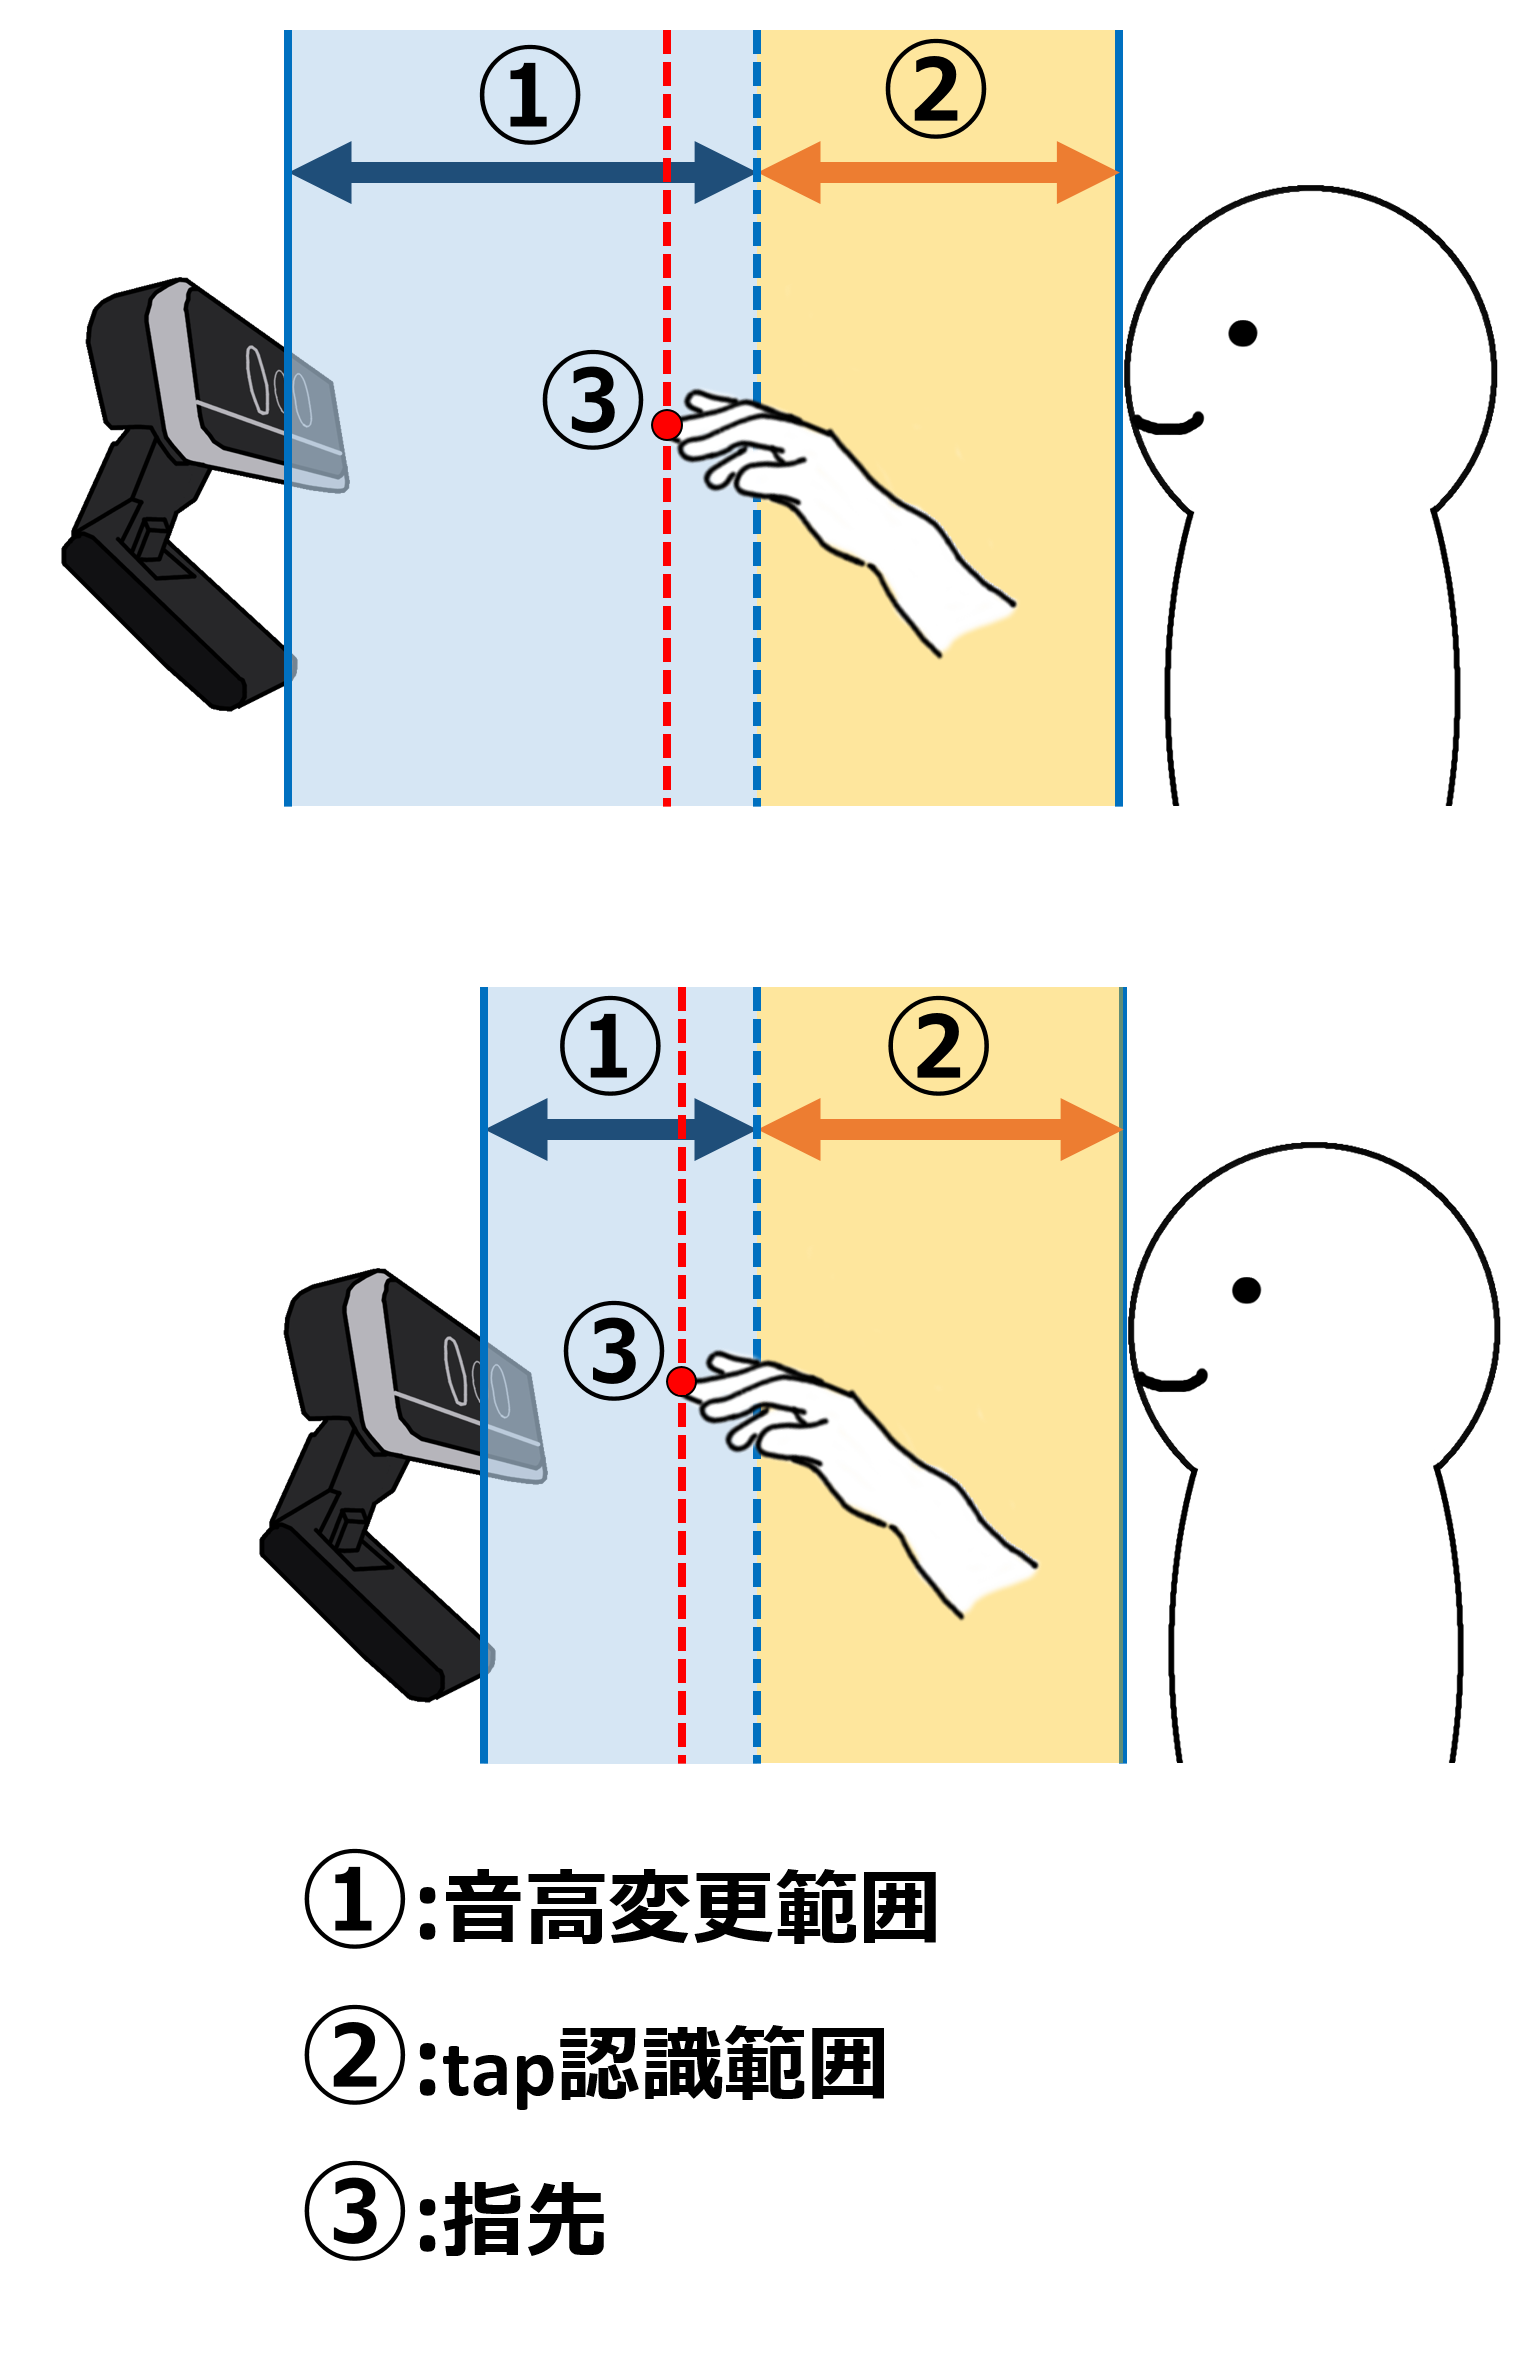
\includegraphics[width=0.9\linewidth]{./pics/04/pitchi_range_change.png}
		\caption{音高変更範囲とtap認識範囲}
		\label{img:range}
	\end{center}
\end{figure}

\section{実行結果と考察}
図\ref{img:red},図\ref{img:blue}に実行結果を示す.音高範囲変更中であることがわかりやすいように指先が音高変更領域に入ったら色のついた円を表示させるようにした.出力範囲は赤,黄,緑,青,紫の順に低くなっていく.この手法によって出力範囲を変更すれば6オクターブ分の範囲の音を出すことができた.これは61鍵(5オクターブ)ピアノの音高範囲より多いのでユーザーが出したい音をカバーできると考えられる.しかし,音高範囲変更中の手は演奏ができないため演奏の自由度が下がるため,なるべく音高変更機能を使わないようにするため,音高範囲の音の数の多さとの一つの音の領域が操作しやすいサイズとなることを両立させた音高範囲の取り方を今後の課題としたい.
\begin{figure}[htbt]
	\begin{center}
		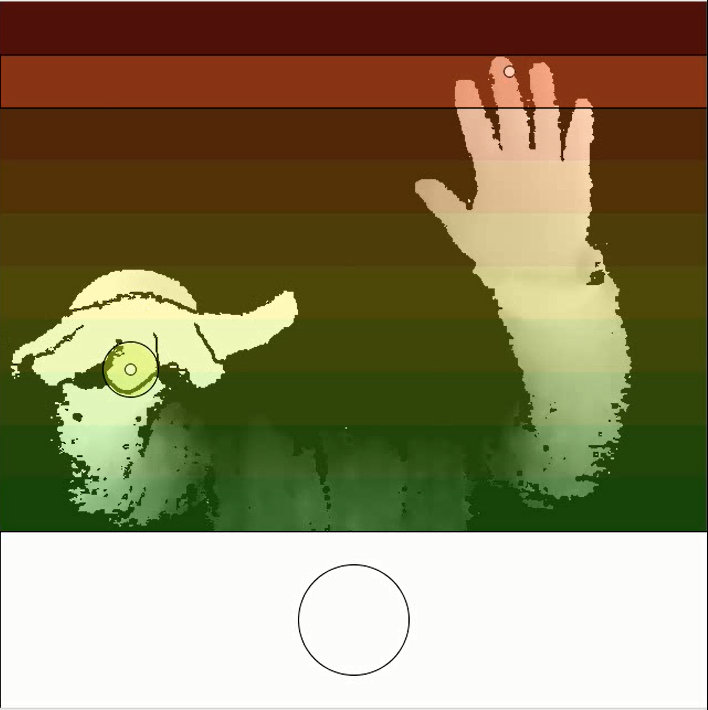
\includegraphics[width=0.5\linewidth]{./pics/04/red.png}
		\caption{出力範囲の変更(高音)}
		\label{img:red} 
	\end{center}
\end{figure}

\begin{figure}[htbt]
	\begin{center}
		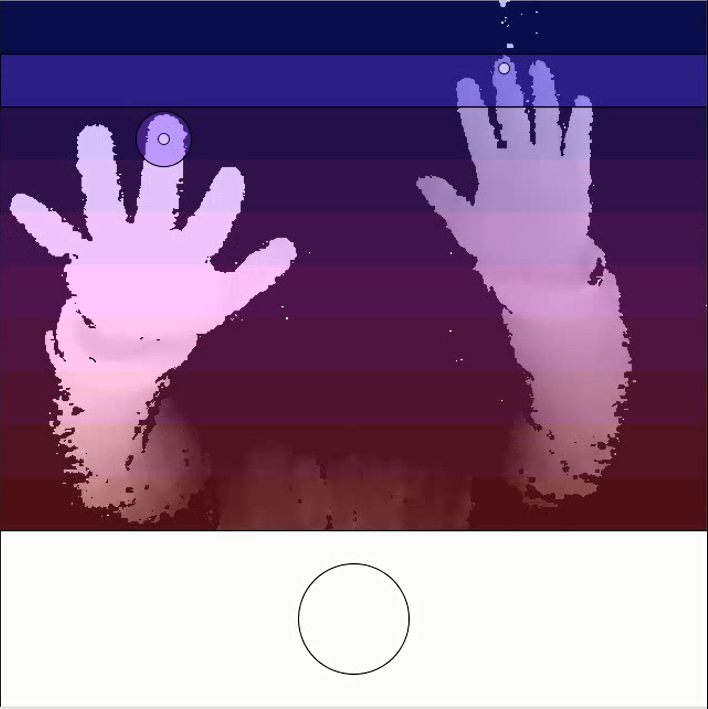
\includegraphics[width=0.5\linewidth]{./pics/04/blue.png}
		\caption{出力範囲の変更(低音)}
		\label{img:blue} 
	\end{center}
\end{figure}
\cleardoublepage

% ツイートの探索的閲覧支援システムの実装
%!TEX root = ../../main.tex
\chapter{調性制約の生成}
本章では調性制約の生成方法について述べる
%--------%---------%---------%--------%---------%---------
\section{調性制約の形式}
調性制約は,曲のコード進行に応じて出力可能な音の周波数列を変化させている.本研究では調性制約は時間(ms),出力可能な周波数列のcsvファイルとして生成され,周波数列の選び方は(1)コードの構成音のみ.(2)コードの構成音+コードに対するメロディ頻度の高い音.の2種類の調性制約を生成した.
\subsection{コードに対するメロディ頻度のカウント}
Songleからのコードとメロディのデータ100曲分を使用してその統計をとる.まず,コードを表\ref{tab:convert}に従って別のコードに分類する.表\ref{tab:convert}は100曲分のコードで出現頻度の高いコードのみを載せている.分類後の各コードのときCからBまでの1オクターブ分12音が流れている時間を計測し,調の主音からの相対的な位置が等しいコードとメロディをまとめてカウントする.例えば,調の主音AのときのコードAでメロディG\#が流れた場合と,調の主音CのときのコードCでメロディBが流れた時は同じ物としてカウントする.こうしてカウントしたメロディのながさの合計(ms)を各コードのメロディ出現頻度とした.メロディの周波数が1オクターブの範囲を超える場合は,オクターブ般化を行ってからカウントする.カウントは長調と短調は分けてカウントした.図\ref{img:MIM},図\ref{img:MIVM},図\ref{img:MVM}にそれぞれ長調のときのコードIM,コードIVM,コードVMのときの各メロディの出現頻度を,図\ref{img:mIM}PFG Tonnetz上に表示したものをそれぞれ示す.
図\ref{img:MIM},図2\ref{img:MIVM},図3\ref{img:MVM}を比べると
コードの根音が5度上にあがるとグラフの平面上でコードの三和音が右に平行移動したが,
5度さがったとき単純な平行移動ではなく根音ではなく主音の頻度のほうが大きい.
構成音以外の音の違いは
根音の左上(6度)右上(7度)を比べると図\ref{img:MIM}、図\ref{img:MIVM}は同じくらいで図\ref{img:MVM}は右上がかなりすくない.
図\ref{img:MIM}と図\ref{img:mIM}を比べると同じコードでもメロディ頻度の分布に違いが生じていて,短調のほうは原点の下側の領域に分布が出やすくなっている.
\subsection{周波数列の決定}
調性制約がもつ(2)の周波数列を決定する時に,コードに対するメロディの出現頻度から決める.コードの構成音に加えて,構成音以外でメロディ頻度が一番高いものを基準にその音に経験的に設定した倍率をかけた値と,コードに対するメロディの割合を閾値としてその閾値を上回った音を周波数列に加える.経験的に設定した倍率や閾値はコード構成音以外の音の頻度を降順にソートして平均をとって設定した.
 \begin{table}[t]
     \caption{コード変換表}
     \begin{center}
         \begin{tabular}{ | c | c || c | c | } \hline
         	変換前 & 変換後 & 変換前 & 変換後 \\ \hline \hline
			XM & XM &Xsus4 & XM \\ \hline
			X-13 & XM & Xadd2 & XM \\ \hline
			X-11 & XM & Xadd4 & XM \\ \hline
			X-9 & XM & Xadd9 & XM \\ \hline
			X-9 & X7 & Xaug & XM \\ \hline
			X-5 & XM & XaugM7 & XM7 \\ \hline
			X-4 & X7 & Xdim & Xm \\ \hline
			X6 & X6 & Xdim7 & Xm \\ \hline
			X7 & X7 & Xm & Xm \\ \hline
			X9 & X7 & Xm11 & Xm7 \\ \hline
			X11 & X7 & Xm13 & Xm7 \\ \hline
			X13 & X7 & Xm6 & Xm \\ \hline
			X7-5 & X7 & Xm7 & Xm7 \\ \hline
			X7-9 & X7 & XM7 & XM7 \\ \hline
			X7-Aug & X7 & Xm7-9 & Xm7\\ \hline
			X9-Aug & X7 & Xm9 & Xm7 \\ \hline
			X9-5 & X7 & XM9 & XM7 \\ \hline
			X7+11 & X7 & Xmadd9 & Xm7 \\ \hline
			X7+13 & X7 & XmM7 & Xm \\ \hline
			X7+9 & X7 & Xsus2 & XM \\ \hline
			X7b5 & X7& Xsus4 & XM \\ \hline
         \end{tabular}
         \label{tab:convert}
     \end{center}
 \end{table}
 
\begin{figure}[t]
	\begin{center}
		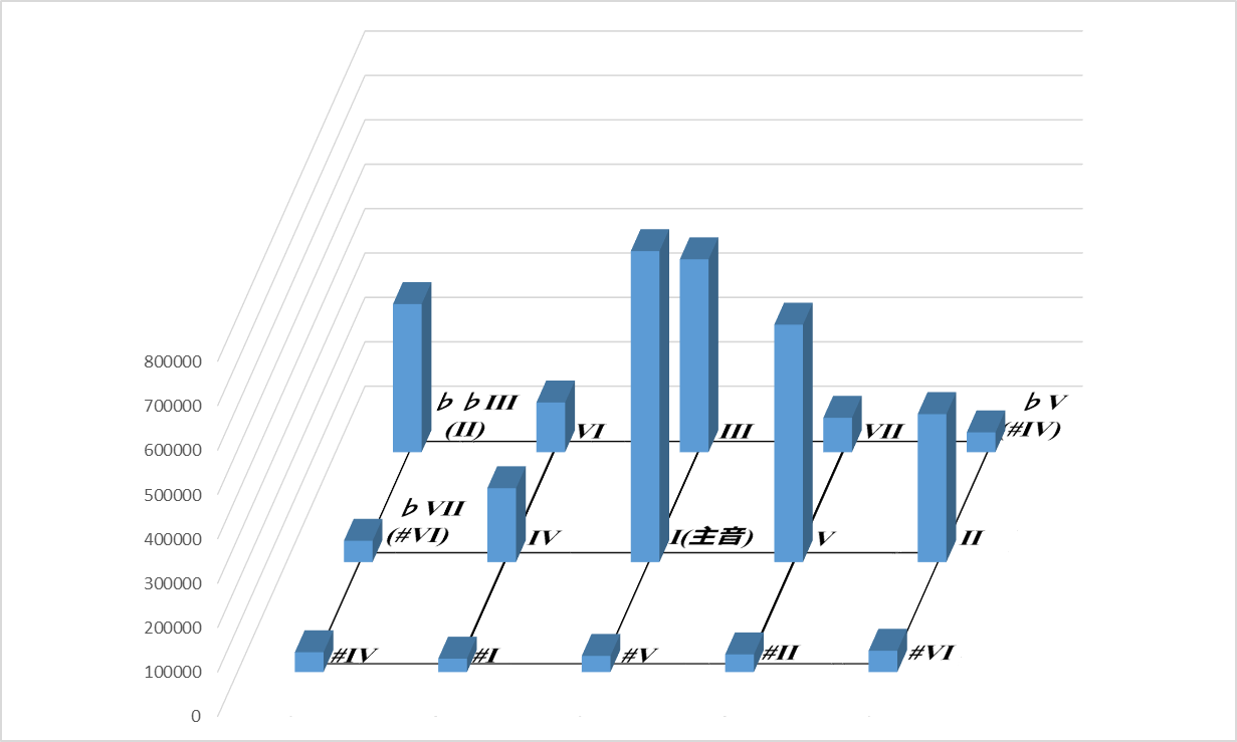
\includegraphics[width=0.8\linewidth]{./pics/05/MajorIM.png}
		\caption{長調のコードIMの各メロディの出現頻度}
		\label{img:MIM} 
	\end{center}
\end{figure}
\begin{figure}[t]
	\begin{center}
		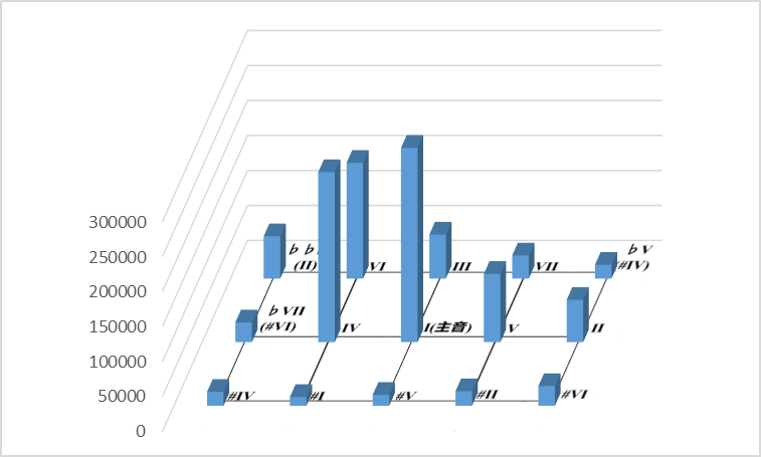
\includegraphics[width=0.8\linewidth]{./pics/05/MajorIVM.png}
		\caption{長調のコードIVMの各メロディの出現頻度}
		\label{img:MIVM} 
	\end{center}
\end{figure}
\begin{figure}[t]
	\begin{center}
		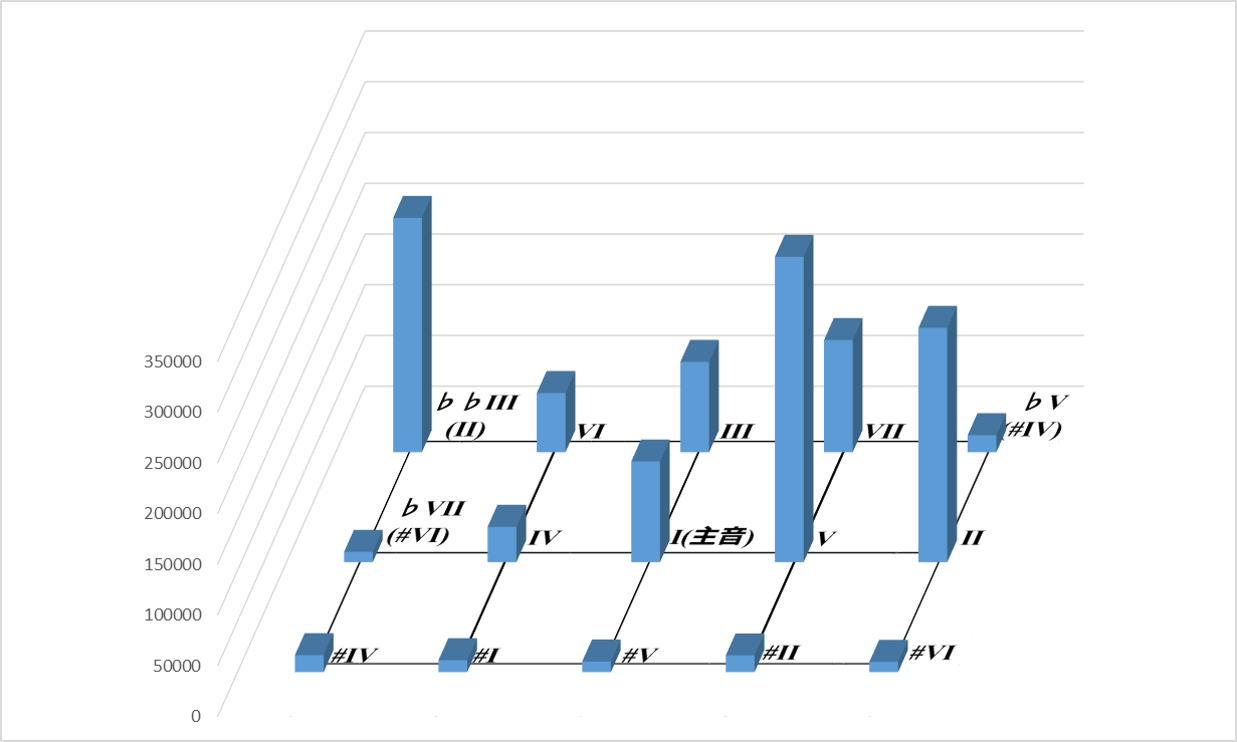
\includegraphics[width=0.8\linewidth]{./pics/05/MajorVM.png}
		\caption{長調のコードVMの各メロディの出現頻度}
		\label{img:MVM} 
	\end{center}
\end{figure}
\begin{figure}[t]
	\begin{center}
		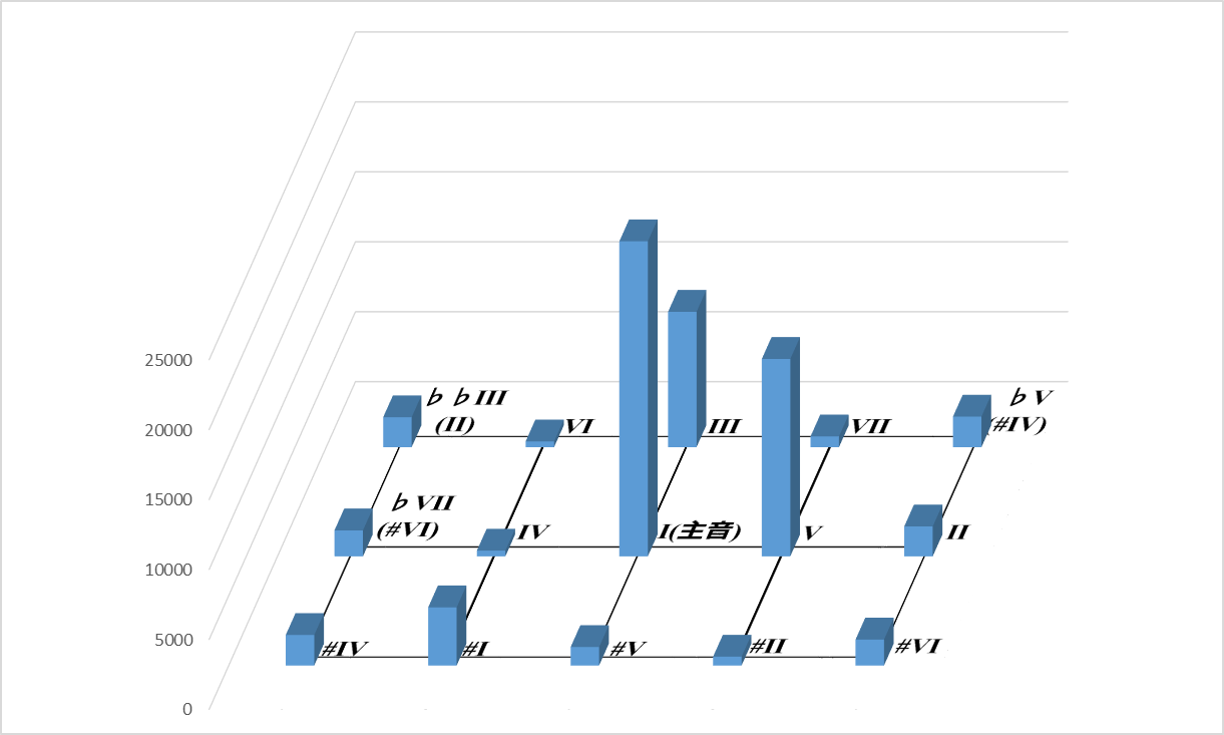
\includegraphics[width=0.8\linewidth]{./pics/05/minorIM.png}
		\caption{短調のコードIMの各メロディの出現頻度}
		\label{img:mIM} 
	\end{center}
\end{figure}
\cleardoublepage

% 評価・考察
%!TEX root = ../../main.tex
\chapter{性能評価・考察}
本研究の評価として,tap認識の精度と調性制約の評価実験を行った.
%--------%---------%---------%--------%---------%---------
\section{実験内容}
20代から50代の男女12人に本システムを実際に体験してもらい,評価用紙の質問に答えてもらう.
%インタフェースの操作に慣れてくると後に操作した手法の評価に影響を受けてしまうおそれがあるため,条件を平等にするため被験者の半分には提案手法のあと比較手法,残り半分には比較手法のあと提案手法の順序で実験をしてもらった.
減衰音を出力するtap動作の認識手法については,第3章で説明した提案手法に対し,RealSense SDKで用意されたデフォルトの認識との比較を行った.調性制約の生成手法については,第5章で説明した提案手法に対し,単純に背景楽曲のコードの構成音を調性制約として用いる手法との比較を行った.ただし,提案手法と比較手法の順序が固定されていると被験者による操作習熟の影響が生じるため,半分の6人は提案手法が先で比較手法が後,もう半分の6人は比較手法が先で提案手法が後になるように,実験を行った.
\subsection{tap評価実験}
第3章で説明したtap認識の提案手法とRealSense SDK で用意されたデフォルトのtap認識の2つの方法で,背景楽曲の拍を表す円に合わせてtapをしてもらい,各実験の後図\ref{img:eval1}の二つの質問に答えてもらった.

\subsection{調性制約評価実験}
コードの構成音のみを周波数列にもつ調性制約と,Songleのデータから統計的に生成した調性制約で演奏してもらい,各演奏の後図\ref{img:eval2}の2つの質問に答えてもらった.

\section{実験結果と考察}
tap評価実験の結果の平均を図\ref{img:result1}に示す.調性制約評価実験の結果の平均を図\ref{img:result2}に示す.図\ref{img:result1}より,本研究で実装したtap認識の方がRealSense SDKのtap認識よりも高い評価を得ているので,実用的であると言える.図\ref{img:result2}より統計的に生成した調性制約は,コードの構成音のみを周波数列にもつ調性制約と比べ不協和音が含まれるが,わずかに意図通りの演奏がしやすいという評価を得た.これはコードの構成音にさらに音を追加したことで表現の幅が広がったためと思われる.不協和音が多いため,追加する音を決める閾値の調節または追加する手法の検討を今後の課題としたい.

\cleardoublepage

% まとめ
%!TEX root = ../../main.tex
\chapter{まとめ}
%--------%---------%---------%--------%---------%---------
\section{本研究の要約}
本研究では直感的にリズムと旋律線を入力すれば背景楽曲との調性を満たす音を出力する演奏インタフェースを実現した.リズムと旋律線はRealSenseカメラを利用して入力し,ジェスチャー認識機能によってインタフェースの操作を行う.RealSense SDKのジェスチャー認識機能には認識漏れや,遅延などが目立ったため,本研究では指先や手のひらの速度や移動距離の閾値,指の開閉度などのパラメータを利用してジェスチャーの認識精度を向上させた.また,深度と身体動作から演奏中に発音可能な音高の範囲を指定できる機能を追加して演奏の自由度をあげた.出力される音はあらかじめSongleから統計的に生成した背景楽曲との調性制約によって決定し,発音可能な周波数列をコード進行に応じて変化させる.特に認識漏れや遅延の多いtap認識の改善と生成した調性制約について,評価実験を行ったところ,改善したtap認識機能はRealSense SDKと比べ実用的な精度であり,調性制約はコードの構成音のみを周波数列とする調性制約より不協和音が多いがわずかに意図通りの演奏がしやすいという評価を得た.
\section{今後の展望}
今後の課題・展望としては機能面において,音量変更機能や,楽器音の出力機能の実装や調性制約の精度向上.マウス,タブレットなどを入力装置とした本システムの実装.ハッカソンなどで簡単に扱えるようAPI化など,他の入力装置への対応や連携の充実化を図りたい.
将来的には,地域社会振興のために開催される音楽イベント,アーティストのコンサートなど多人数で同時に即興合奏ができるように,複数人の身体動作入力の処理,画面を見ないでも操作できるような直感的な操作,オンラインで離れた人と合奏などを今後の課題としたい.
\cleardoublepage

% 謝辞
%!TEX root = ../../main.tex
\chapter*{謝辞}
\addcontent{謝辞}
本論文を執筆するにあたり,多くの方のご支援ご協力を賜りました.この場で皆様に感謝の言葉を申し上げたいと思います.

まず,名古屋工業大学大学院 工学研究科 情報工学専攻の白松~俊准教授に厚く御礼申し上げます.白松教授には日々の研究活動に限らず,音楽知識の乏しい私に懇切丁寧にご指導して頂き,数多くの貴重な体験もさせて頂きました.ここに心より感謝致します.

%京都大学 糸山~克寿助教授,吉井 和佳講師には,研究方針や実装に関して親身にご指導して頂き,非常に多くの有益なご意見を頂きました.の助言により本研究が飛躍的に進展しました.ここに心より感謝致します.

同研究室の同輩である成瀬~雅人君,西田~拓哉君,山野~太靖君とは特に苦楽を共にしてきました.
その中で,皆の頑張り,励まし,助言に助けられることも多く,充実した日々を過ごすことができました.ここでみなさんに感謝の意を表しつつ,今後のご活躍をお祈り申し上げます.

その他,バイト先のとだがわこどもランドの皆様をはじめ,多数の友人たちにも評価実験の協力をして頂きました.ここで合わせて御礼申し上げます.

最後に,研究活動で帰りが遅くなることもあり迷惑をかけた私を,いつもと変わらず支えてくれた家族に,心より感謝致します.

\vspace*{4.5mm}

\begin{flushright}
%思い出で溢れている 白松研究室にて \\
%2016年 桜咲く頃に \\
\vspace*{1.8mm}
\end{flushright}
\cleardoublepage

% 参考文献
%!TEX root = ../../main.tex
%修論用
% 参考文献 http://bibdesk.sourceforge.net/manual/BibDesk%20Help_94.html#SEC179 による出力
%以下テンプレ
%<$publications>
%\bibitem{<$citeKey/>}
%<$authors.name.stringByRemovingTeX.@componentsJoinedByComma/>: ``<$fields.Title.stringByRemovingTeX/>,''  <$fields.Journal.stringByRemovingTeX/>. Vol. <$fields.Volume/>,  No. <$fields.Number/>,  pp. <$fields.Pages/>,  <$fields.Year/>.
%<$fields.URL/>
%<$fields.localURL/>
%\begin{quote}
%\end{quote}

%
%</$publications>
\addcontent{参考文献}

\begin{thebibliography}{99}
% メディアについて

\bibitem{hatano2007}
波多野誼余夫(編):"音楽と認知" Vol. 8, 東京大学出版会, (2007)
\begin{quote}
様々な認知研究や音楽理論から音楽心理学を,人間はいかにして音楽を認知するかの研究として捉えて考察をのべている.
\end{quote}

\bibitem{songle}
能動的音楽鑑賞サービスSongle,\url{http://songle.jp/},2015年11月25日アクセス.
\begin{quote}
	能動的音楽鑑賞サービスSongleは動画サイトやネット上にアップロードされた合法的に視聴できる音楽を自動解析し,音楽と一緒にサビ,メロディ,コード,ビートを視覚的に表示させて鑑賞することができる.
\end{quote}

\bibitem{ongakunotomo1979}
音楽之友社:"音楽中辞典" 音楽之友社, (1979)
\begin{quote}
音楽用語の解説・用法を記載した辞典.
\end{quote}

\bibitem{suga2008}
菅道子. "身体表現を取り入れた参加型音楽コンサートの可能性: カノンの理解を目指した 「追いかけっこしよう」 の事例から" 和歌山大学教育学部教育実践総合センター紀要 18 , pp. 121-129, (2008)
\begin{quote}
	音楽理解における身体表現の有効性を小学校低学年を対象とした参加型音楽コンサートの企画・実施を通して検討し,旋律線のてなぞりなどの身体動作が音楽理解を促進することをあげている.
\end{quote}

\bibitem{takahasi2010}
高橋祐樹:"私の研究開発ツール Processing" 映像情報メディア学会誌 Vol. 64, No.12, pp. 1841-1849, (2010)
\begin{quote}
	Processingの説明と,基本的な使い方について述べている.
\end{quote}

\bibitem{nakamura2010}
中村俊介, 竹井将紫: "インタラクティブアート 「KAGURA」 によるワークショップ: 東京ミッドタウン・デザインハブ・キッズウィークにおける子供向けイベントの報告 (B-2 音楽と聴覚のデザイン, 研究発表, 芸術工学会 2010 年度秋期大会 in 浜松)."  芸術工学会誌,  Vol. 54, pp. 48-49, (2010)
\begin{quote}
カメラの前で動いて音声を生成するインタラクティブアート「KAGURA」をデジタルでしかできないインタラクティブな教育コンテンツとして利用しようと考え,東京ミッドタウンで開催された小・中学生向けワークショップで展示したときの報告が書かれている.
\end{quote}

\bibitem{kagura}
KAGURA,\url{http://www.kagura.cc/jp/},2015年11月25日アクセス
\begin{quote}
	Real Senseに対応した身体動作とジェスチャーで操作できる音楽演奏アプリケーション.
\end{quote}

\bibitem{kanke2013}
菅家浩之, 竹川佳成, 寺田努, 塚本昌彦:"Airstic Drum: 実ドラムと仮想ドラムを統合するためのドラムスティックの構築" 情報処理学会論文誌, Vol. 54, No. 4, pp. 1393-1401, (2013)
\begin{quote}
	楽器の運搬と演奏スペースの問題を解決するため,使用頻度の低い打楽器に仮想的なドラムを割り当て加速度センサの閾値から仮想ドラムの叩打と実ドラムの叩打を区別する方法について述べている.
\end{quote}

\bibitem{shiramatsu2015}
Shiramatsu, S., Ozono, T., and Shintani S.: A Computational Model of Tonality Cognition Based on Prime Factor Representation of Frequency Ratios and Its Application. Proc. of SMC 2015, (2015)
\begin{quote}
	調性理解モデルPFG Tonnetzについて述べている.
\end{quote}

\bibitem{behringer10}
Behringer, R. and Elliot, J.: Linking Phys- ical Space with the Riemann Tonnetz for Exploration of Western Tonality, chapter 6, pp. 131–143, Nova Science Publishers, (2010)
\begin{quote}
	1880年にRiemannが発展させたTonnetzを分析し,数式化した.
\end{quote}
%
%\bibitem{hewlett07}
%Hewlett, W., Selfridge-Field, E., and Cor- reia, E.: Tonal Theory for the Digital Age, Vol. 15 of Computing in Musicology, Center for Computer Assisted Research in the Humanities, Stanford University, (2007)
%\begin{quote}
%	
%%\end{quote}
%
%\bibitem{tymoczko12}
%Tymoczko, D.: The Generalized Tonnetz, Journal of Music Theory, Vol. 56, No. 1, pp. 1–52, (2012)
%\begin{quote}
%	
%\end{quote}

\bibitem{hand_labels}
Intel RealSense SDK 2015 R5 Documentation, \url{https://software.intel.com/sites/landingpage/realsense/camera-sdk/v1.1/documentation/html/index.html?jointtype_pxchanddata.html}, 2016年1月25日アクセス
\begin{quote}
	RealSenseが認識できる関節の種類が載っている.
\end{quote}

\end{thebibliography}
\cleardoublepage

\appendix
%!TEX root = ../../main.tex
\cleardoublepage
\chapter{平成27年度 電気・電子・情報関係学会 東海支部連合大会}
\begin{figure}[ht]
    \begin{center}
        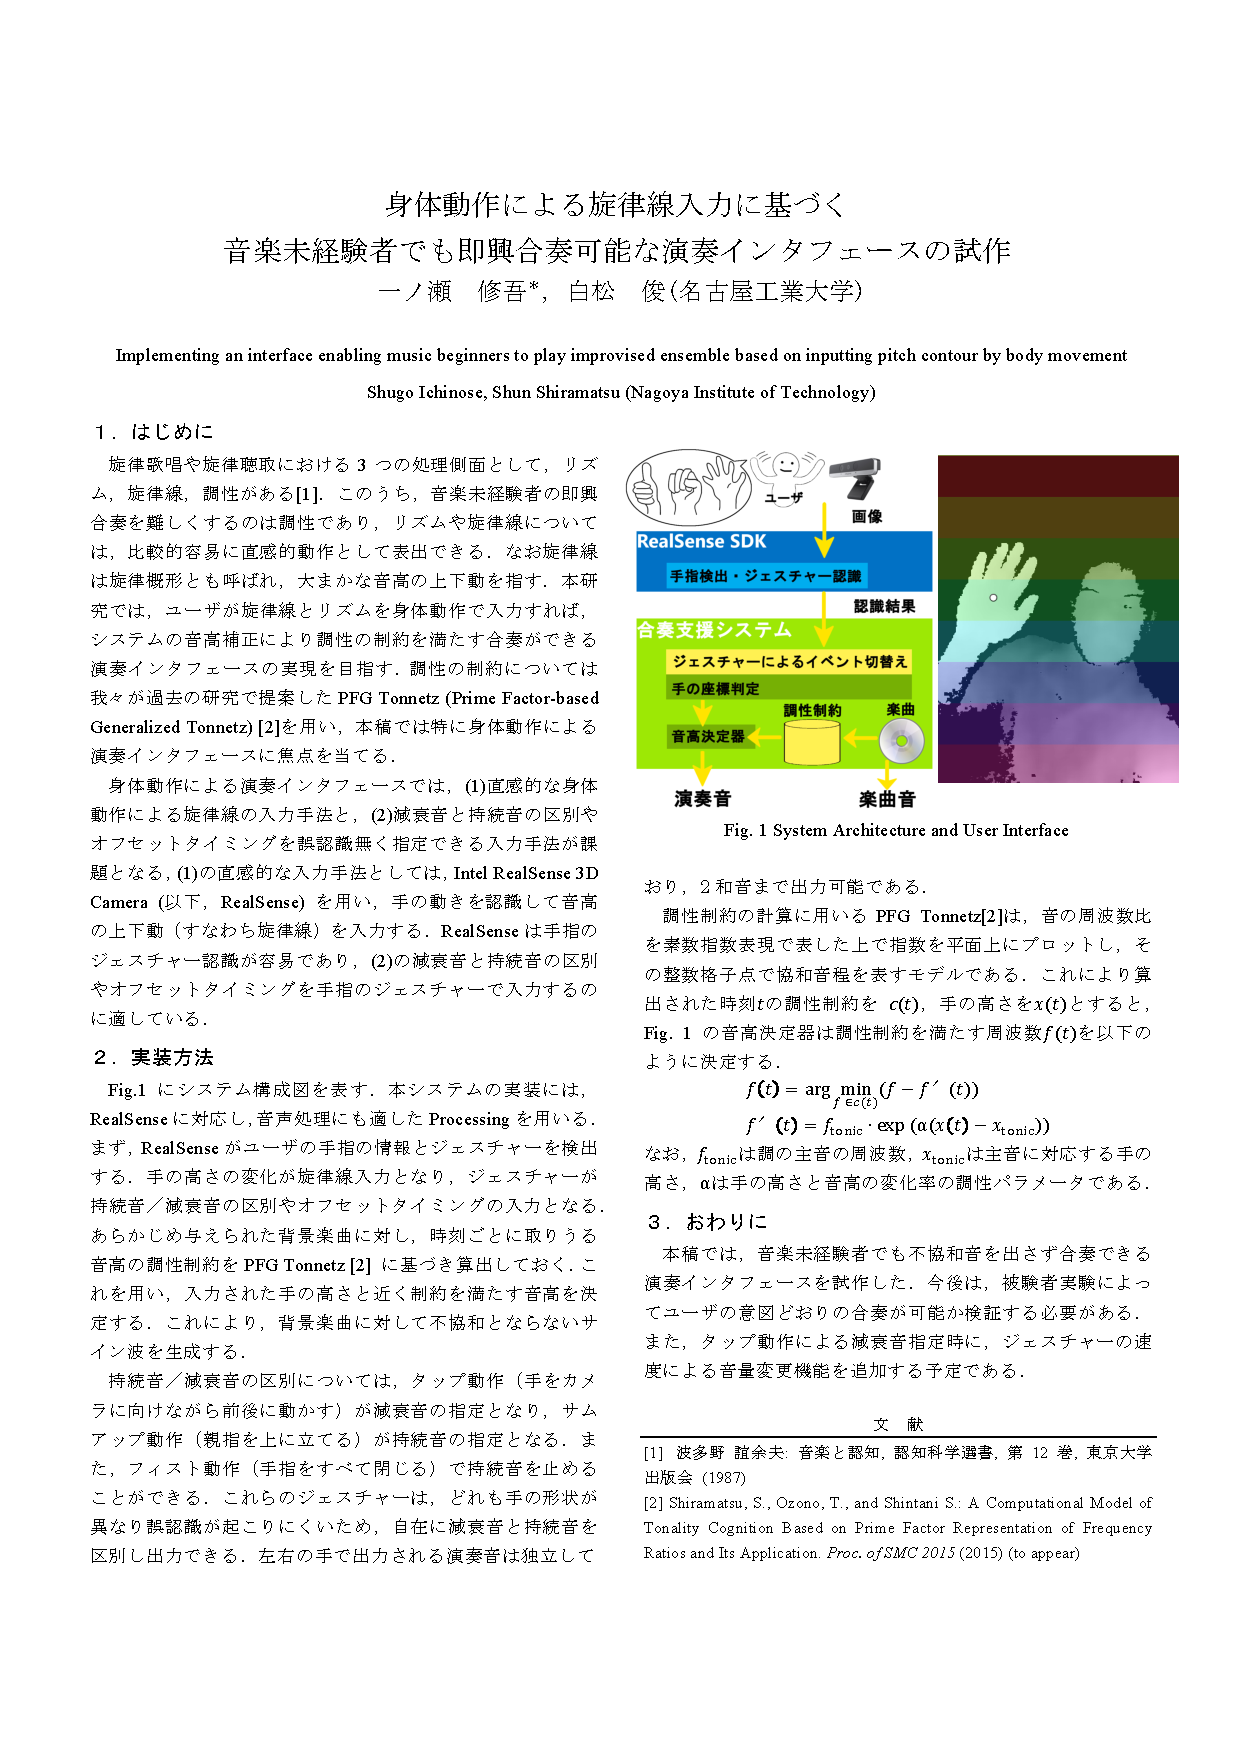
\includegraphics[width=1.0\linewidth]{part/A.IPSJrengou2014/ichinose2015tokai0717.pdf}
    \end{center}
\end{figure}

\clearpage

%!TEX root = ../../main.tex
\cleardoublepage
\chapter{IPSJ2016\\第78回情報処理全国大会(掲載予定)}

\begin{figure}[ht]
    \begin{center}
        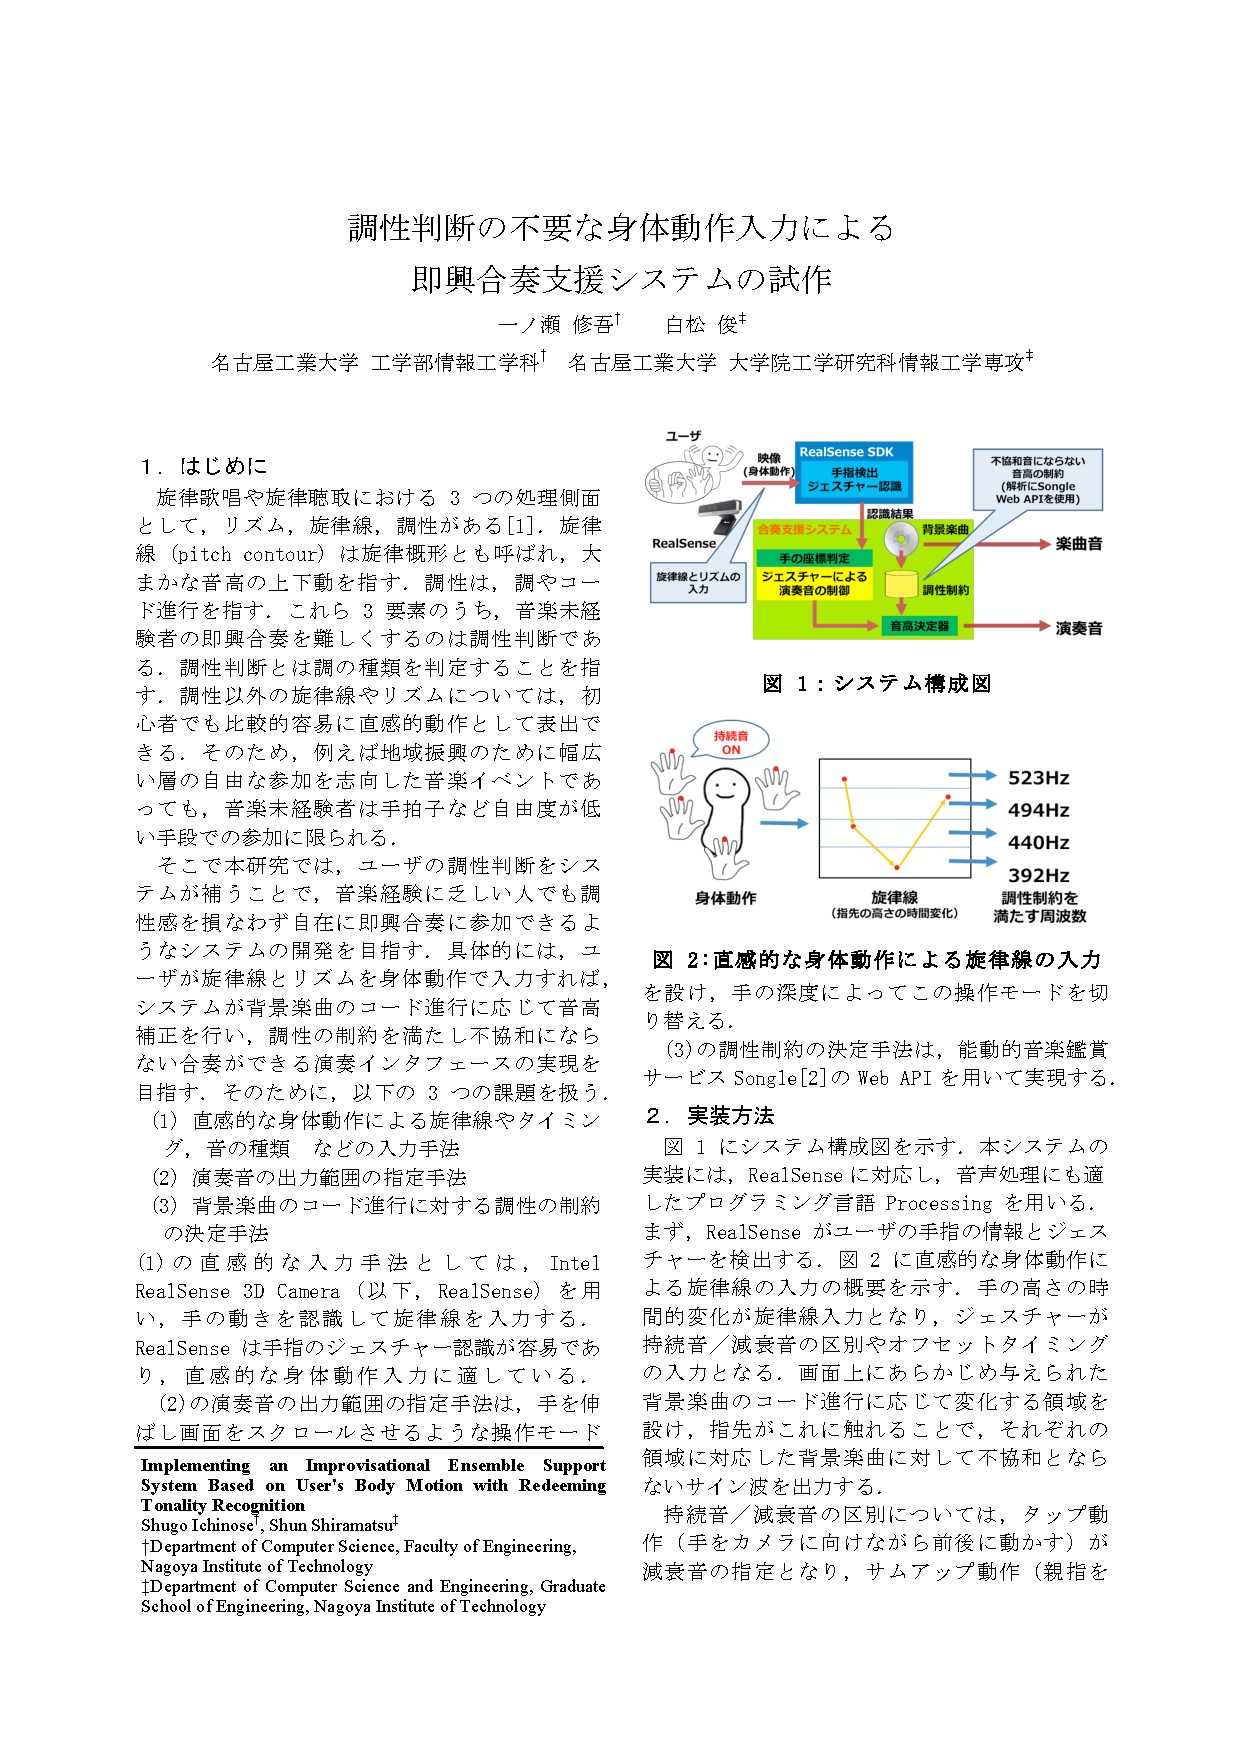
\includegraphics[width=1.0\linewidth]{part/B.IPSJ2015/ichinose160105_1.pdf}
    \end{center}
\end{figure}

\newpage
\clearpage

\begin{figure}[ht]
    \begin{center}
        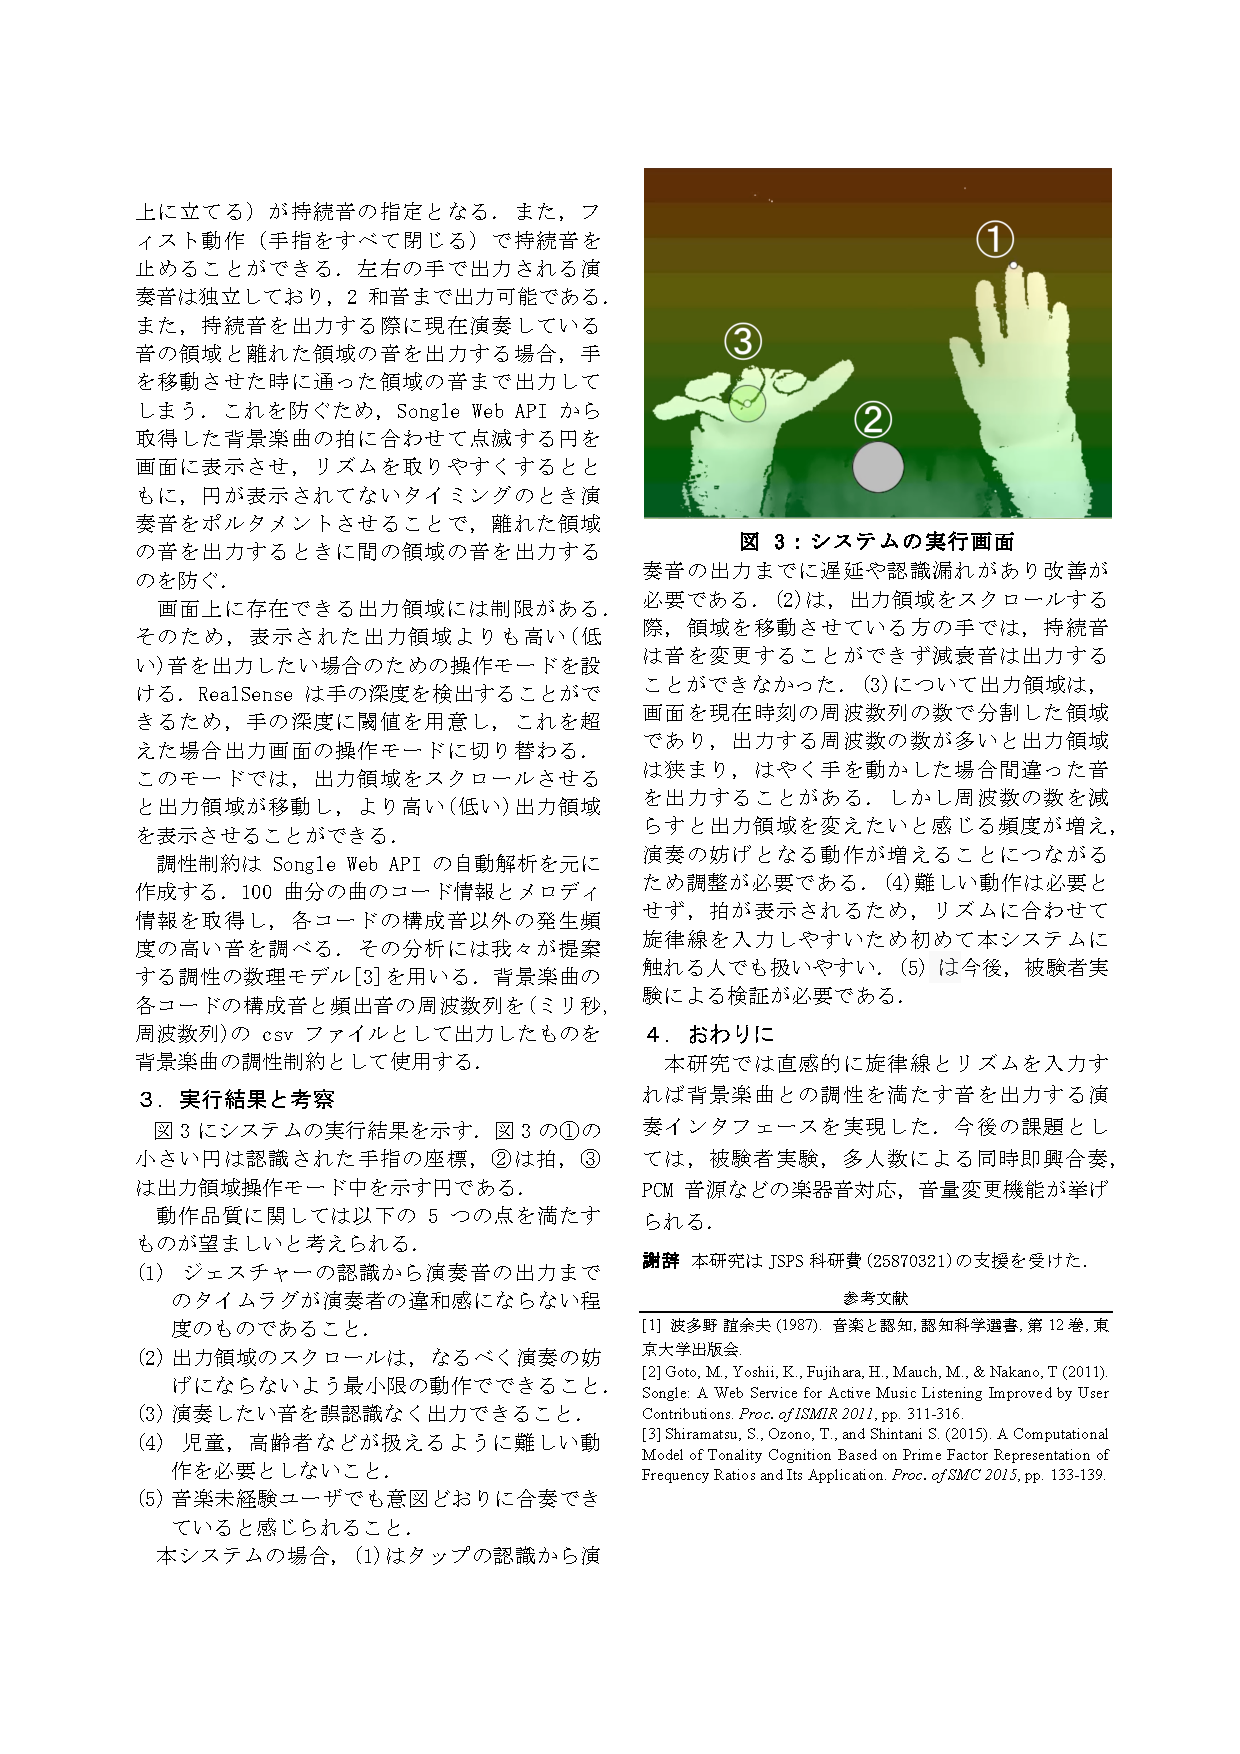
\includegraphics[width=1.0\linewidth]{part/B.IPSJ2015/ichinose160105_2.pdf}
    \end{center}
\end{figure}

\clearpage


\cleardoublepage
%!TEX root = ../../main.tex
% タイトルページ
%\documentclass[a4j,12pt]{jreport}
%\usepackage{graphicx}
%\usepackage{times}
%\usepackage{selectp}
%\usepackage{epsf}
%\usepackage{epsbox}
%\usepackage{graphicx}
%\usepackage{verbatimfiles}
%\usepackage{here}
%%\usepackage{url}
%\usepackage{fancyhdr}
%\usepackage{algorithm}
%\usepackage{cite}
%\usepackage{ascmac}
%\usepackage{amsmath}
%\usepackage{amsthm}
%\usepackage{amssymb}
%\usepackage{latexsym}

%\usepackage{thesis}
%\input{mymacros}

%\oddsidemargin=17mm
%\evensidemargin=-4mm

%\setlength{\textwidth}{40zw}
%\begin{document}

\thispagestyle{empty}
\setcounter{page}{0}

%%%%%%%%%%%%%%%%%%%%%%%%%%%%%%%%%%%%%%%%%%%%%%%%%
% 定義
%%%%%%%%%%%%%%%%%%%%%%%%%%%%%%%%%%%%%%%%%%%%%%%%%

% タイトル
\def \title{MissionForest: 組織内外における\\協働支援のためのタスク構造化システムの試作}

% 著者
\def \author{後藤~誉昌}

% 提出日
\def \date{\today}

% 指導教官名
\def \teacher{白松~俊}

% 指導教官の肩書き
\def \teacherrank{准教授}

% 所属
\def \belong{名古屋工業大学\\工学部 情報工学科}

% 入学年度
\def \year{23}

% 学籍番号
\def \regnum{24115054}

%%%%%%%%%%%%%%%%%%%%%%%%%%%%%%%%%%%%%%%%%%%%%%%%%
% 本文
%%%%%%%%%%%%%%%%%%%%%%%%%%%%%%%%%%%%%%%%%%%%%%%%%

\def\sizeLL#1{\Huge #1}
\def\sizeL#1{\LARGE #1}
\def\sizeM#1{\Large #1}
\def\sizeS#1{\large #1}

\def\REYrule{\hbox to 5cm{\leaders\hrule height 1pt\hfill}}
\newbox\REYbox
\def\announce#1{
  \setbox\REYbox=\hbox{\REYrule\quad{\Large\bf #1}\quad\raise3pt\REYrule}%
  \gdef\REYbigrule{\hbox to \wd\REYbox{\leaders\hrule height 1pt \hfill}}%
  \centerline{\raise3pt\REYrule\vspace*{2mm}\quad{\LARGE #1}\quad\raise3pt\REYrule}}
\def\endannounce{\par\centerline{\REYbigrule}}

\begin{titlepage}
 \begin{center}
 %\renewcommand{\baselinestretch}{1.0}
  \vspace*{5mm}
  \sizeLL{卒業論文}\\
  \vspace*{10mm}
  \begin{announce}{(題~~目)}
   \sizeL{\title}\\
  \end{announce}
  \vspace*{20mm}
  \sizeM{指導教員~~~~~}\sizeL{\teacher}\sizeM{~~\teacherrank}\\
  %\vspace*{40mm} % 題目が2行の場合
 % \vspace*{30mm} % 題目が3行の場合
 \vspace{10mm}
  \sizeM{\belong}\\
  \vspace*{10mm}
  \sizeM{平成 \year 年 4 月 入学}\\
  \vspace*{3mm}
  \begin{table}[H]
    \begin{center}
     \begin{tabular}{cl}
      \sizeM{(学籍番号)} & \sizeL{{\underline{~~ \regnum ~~}}} \\
      \sizeM{(氏~名)} & \sizeL{\underline{~~ \author ~~}} \\
     \end{tabular}
    \end{center}
   \end{table}
  \vspace*{10mm}
  \sizeS{(提出日:~\today)}
  % \sizeS{(提出日:\ ~平成28年2月8日)}
 \end{center}
\end{titlepage}

%\end{document}


\end{document}
